%---------------------------------------------------------------
\chapter{\babTiga}
%---------------------------------------------------------------

%-----------------------------------------------------------------------------%
\section{Sistem Arsitektur}
%-----------------------------------------------------------------------------%

Perancangan sistem arsitektur aplikasi sistem pengawakan jabatan struktural dapat dilihat pada \textbf{Gambar 3.1.} berikut : 

\begin{figure}
	\centering
	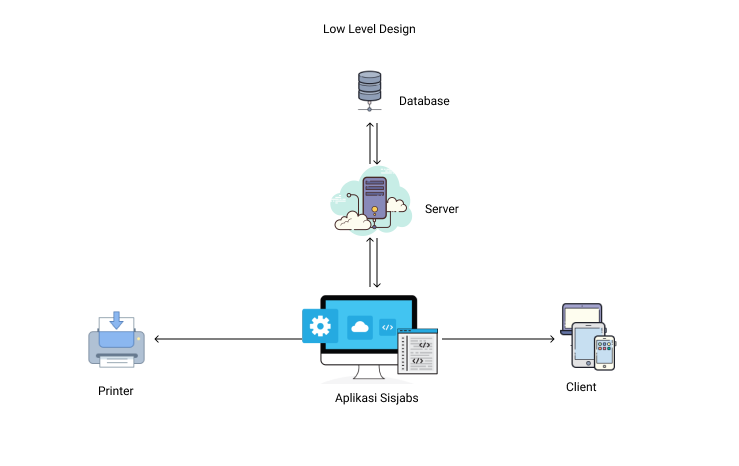
\includegraphics[width=1\textwidth]
	{pics/LowLevelDiagram.png}
	\caption{Low Level Design}
	\label{fig:31}
\end{figure}


\subsection{Gambaran Umum Sistem}

Aplikasi \textbf{SiPJabS : Sistem Pengawakan Jabatan Struktural di Univertias Telkom} merupakan aplikasi berbasis web yang memudahkan bagi perusahaan dalam pencarian seorang kandidat atau posisi yang kosong. Dalam pembuatan aplikasi ini dibutuhkan fitur \textit{filtering} yang digunakan untuk pencarian kandidat baru, yang sesuai dengan ketentuan yang sudah ditetapkan oleh perusahaan. Sistem \textit{filtering} dapat dilakukan setiap saat, untuk menggantikan pekerjaan lama yang telah berhenti dikarenakan pensiun, meninggal, mengundurkan diri atau diberhentikan karena suatu kebijakan tertentu. \\

Data-data pegawai yang berada di Universitas Telkom dapat dilihat dan data tersebut bersifat rahasia. Sehingga aplikasi ”\textbf{SiPJabS : Sistem Pengawakan Jabatan Struktural di Universitas Telkom}” hanya dapat diakses oleh orang tertentu. Aplikasi ini terdapat satu \textit{user} yang dapat mengelola proses \textit{filtering} dan satu \textit{admin} yang mengelola infrastruktur \textit{database} dan proyek \textit{server} serta jaringan.  

Sistem \textit{filtering} pada apliaksi ini terbagi menjadi dua bagian, yang pertama merupakan \textit{fitering} secara umum dengan isi \textit{form} seperti jabatan minimal dan masa kerja. Yang kedua merupakan \textit{filtering} secara khusus, dimana \textit{user} dapat mencari kandidat dengan syarat yang lebih spesifik lagi untuk dijadikan pilihan, kemudian akan terdapat beberapa nama kandidat, apabila sudah menentukan pilihan dapat menekan tombol button pada nama yang akan dipilih dan akan masuk dalam \textit{cart} kandidat.

Apabila proses pencarian kandidat sudah ditemukan dengan salah satu proses \textit{filtering} yang sudah dijelaskan diatas maka, proses selanjutnya akan masuk dalam pembuatan berita acara dan dapat dicetak berupa file pdf.  

\subsection{Target Pengguna Aplikasi}

Aplikasi \textbf{SiPJabS} memiliki beberapa target pengguna diantaranya sebagai berikut :

\begin{enumerate}
\item User \\
User merupakan pegawai Direktorat Sumber Daya Manusia Universitas Telkom yang membutuhkan kandidat dengan proses \textit{filtering} untuk mengisi posisi yang kosong atau digantikan.

\item Admin \\
Admin merupakan pegawai Direktorat Pusat Teknologi Informasi Universitas Telkom yang mengelola dan menyediakan data untuk proses filtering.
\end{enumerate}

\subsection{Spesifikasi Target Perangkat}

Spesifikasi dari target perangkat untuk mengakses aplikasi SiPJabS adalah sebagai berikut : 

\begin{enumerate}

\item Komputer atau laptop yang terhubung dengan koneksi internet dan dapat membuka \textit{browser}.

\item	\textit{Smartphone} atau tablet yang terhubung dengan koneksi internet dan dapat membuka \textit{browser}.
\end{enumerate}

\subsection{Diagram Alir Aplikasi}

Dalam membangun aplikasi SiPJabS, dibutuhkan diagram alir untuk membantu developer dan pengguna dalam memahami sistem yang akan dibuat. Berikut merupakan flowchart :

\begin{figure}
	\centering
	\includegraphics[width=1\textwidth]
	{pics/diagram/flowchart.png}
	\caption{Flowchart}
	\label{fig:31}
\end{figure}  

\newpage
%-----------------------------------------------------------------------------%
\section{Kebutuhan Pengembangan Sistem}
%-----------------------------------------------------------------------------%

Dalam membangun aplikasi \textbf{SiPJabS}, dibutuhkan beberapa perangkat untuk mengimplementasikannya. Perangkat tersebut dibagi menjadi tiga, yaitu perangkat keras (hardware), perangkat lunak (software) dan hosting. Adapun kebutuhan pengembangan sistem adalah sebagai berikut : 

\subsection{Kubutuhan Perangkat Keras (Hardware) }

\textit{Hardware} yang dibutuhkan dalam perancangan dan pembuatan aplikasi SiPJabs
adalah sebagai berikut :


\begin{table}[H]
	\centering
	\caption{Tabel Kebutuhan Hardware}
	\begin{tabular}{ | c | l | p{75mm} | }
		\hline
		No. & Perangkat Keras & Spesifikasi \\
		\hline
		\multirow{6}{*}{1} & \multirow{6}{*}{Laptop MSI GL62M} & Processor : Intel Core i7-7700HQ \\
		& & Operating sistem : Windows 10 Education \\
		& & RAM : 8 GB \\
		& & Storage : 128 GB SSD + 1 TB Hardisk \\
		& & Graphics Card :  nVidia Geforce GTX 1050 \\
		& & Display : 15.6" FHD, Anti-Glare (1920 x 1080) \\
		
		
		\hline
		
		\multirow{6}{*}{2} & \multirow{6}{*}{Laptop HP Pavilion x360} & Processor : Intel Core i3-6100U \\
		& & Operating sistem : Windows 10 Home \\
		& & RAM : 12 GB \\
		& & Storage : 500 GB Hardisk\\
		& & Graphics Card : Intel HD 520 Graphics \\
		& & Display : 13.3" HD, Touch Screen \\
		
		\hline
	\end{tabular}
\end{table}


\newpage
\subsection{Kebutuhkan Perangkat Lunak (Software)}

\textit{Software} yang dibutuhkan dalam perancangan dan pembuatan aplikasi SiPJabs
adalah sebagai berikut :

\begin{table}[H]
	\centering
	\caption{Tabel Kebutuhan Software}
	\begin{tabular}{ | c | l | p{65mm} | }
		\hline
		No. & Perangkat Lunak & Kegunaan \\
		\hline
		
		1 & Visual Studio Code & Text editor untuk menuliskan \textit{coding} aplikasi \\
				
		\hline
		
		2 & XAMPP & Sebagai server yang berdiri sendiri, yang terdiri atas program Apache HTTP Server, MySQL database, dan penerjemah bahasa yang ditulis dengan bahasa pemrograman PHP dan Perl \\
		
		\hline
		
		3 & IBM Rational System Architect  & Sebuah software untuk mendesain rancangan sistem aplikasi \\
		
		\hline
		
		4 & Figma & Untuk mendesai user interface secara online \\
		
		
		\hline
		
		5 & Microsoft Office Word & Untuk membuat dokumen dan laporan \\
		
		\hline
		
		6 & TexStudio & Untuk membuat laporan dalam latex \\
		
		\hline
		
		7 & Adobe Premier Pro & Editing vidio demo dan vidio promosi \\
		
		\hline
		
		8 & Brave dan Mozila Firefox & Web browser \\
		
		\hline
	\end{tabular}
\end{table}

\subsection{Kebutuhan Hosting}

\textit{Hosting} yang dibutuhkan dalam perancangan dan pembuatan aplikasi SiPJabs
adalah sebagai berikut :

\begin{table}[H]
	\centering
	\caption{Tabel Kebutuhan Hosting}
	\begin{tabular}{ | c | l | l | }
		\hline
		No. & Server & Spesifikasi \\
		\hline
		\multirow{5}{*}{1} & \multirow{5}{*}{Server Indonesia} & Storage : 2 GB \\
		& & RAM : 1 GB \\
		& & Bandwith : Unlimited \\
		& & Processor : 1 Core \\
		& & Domain : my.id  \\
	
		\hline
	\end{tabular}
\end{table}

%-----------------------------------------------------------------------------%
\section{Perancangan Model Program}
%-----------------------------------------------------------------------------%
Perancangan model program dalam pembuatan aplikasi SiPJabS antara
lain Use Case Diagram, Use Case Skenario, Class Diagram,
Entity Relationship Diagram (ERD). Adapun perancangan model program adalah sebagai berikut :

\subsection{Use Case Diagram}

\begin{figure}
	\centering
	\includegraphics[width=1\textwidth]
	{pics/diagram/usecase.png}
	\caption{Use Case Diagram}
	\label{fig:32}
\end{figure}


\subsection{Use Case Skenario}
Berikut merupakan use case scenario dalam pembuatan aplikasi SiPJabS :

\begin{enumerate}
	\item Skenario Login
	
	Nomor \kern 3.6pc : SP-01 \\
	Nama Use Case : Melakukan login \\
	Aktor \kern 4.1 pc : Admin \\
	Tipe \kern 4.6pc : Primary \\
	Tujuan \kern 3.6pc : Penggunaan aplikasi \\
	Deskripsi \kern 2.5pc : 
	
	\begin{itemize}
		\item Admin dapat menginputkan username dan password
		\item Sistem akan mencocokkan data
		\item Sistem menampilkan halaman utama aplikasi
	\end{itemize}

	\begin{table}
		\caption{Skenario Login}
		\centering
		\begin{tabular}{ | p{55mm} | p{60mm} |}
			\hline 
			\textbf{Aktor} & \textbf{Sistem} \\
			\hline
			
			1.	Menginputkan username dan password &  \\
			
			\hline
			
			& 2. Mencocokkan data \\
			
			\hline
			
			& 3.	Menampilkan halaman utama aplikasi \\
		
			\hline
			
		\end{tabular}
	\end{table}

\item Skenario Edit Profile

Nomor \kern 3.6pc : SP-02 \\
Nama Use Case : Melakukan edit profile \\
Aktor \kern 4.1 pc : Admin \\
Tipe \kern 4.6pc : Primary \\
Tujuan \kern 3.6pc : Admin dapat melakukan edit pada profile \\
Deskripsi \kern 2.5pc : 

\begin{itemize}
	\item Admin menuju ke halaman profile
	\item Sistem akan menampilkan halaman profile
	\item Admin memilih edit profile
	\item Sistem menampilkan pop-up form edit profile
	\item Admin menginputkan data
	\item Admin menyimpan perubahan

\end{itemize}

\begin{table}
	\caption{Skenario Edit Profile}
	\centering
	\begin{tabular}{ | l | l |}
		\hline 
		\textbf{Aktor} & \textbf{Sistem} \\
		\hline
		
		1.	Menuju ke halaman profile &  \\
		
		\hline
		
		&  2.	Menampilkan halaman profile \\
		
		\hline
		
		 3. Memilih edit profile & \\
		
		\hline
		
			& 4.	Menampilkan pop-up form edit profile \\
		
		\hline
		
		5.	Menginputkan data  & \\
		\hline
		
		6.	Menyimpan perubahan & \\
		\hline
		
		& 7.	Menyimpan perubahan \\
		\hline
		
	\end{tabular}
\end{table}

\item Skenario Reset Password

Nomor \kern 3.6pc : SP-03 \\
Nama Use Case : Melakukan reset password \\
Aktor \kern 4.1 pc : Admin \\
Tipe \kern 4.6pc : Primary \\
Tujuan \kern 3.6pc : Admin dapat melakukan reset password pada profile \\
Deskripsi \kern 2.5pc : 

\begin{itemize}
	\item Admin menuju ke halaman profile
	\item Sistem akan menampilkan halaman profile
	\item Admin memilih reset password
	\item Sistem menampilkan pop-up reset password
	\item Admin menginputkan password
	\item Admin menyimpan perubahan
	\item Sistem menyimpan perubahan
	
\end{itemize}

\begin{table}
	\caption{Skenario Reset Password}
	\centering
	\begin{tabular}{ | l | l |}
		\hline 
		\textbf{Aktor} & \textbf{Sistem} \\
		\hline
		
		1.	Menuju ke halaman profile &  \\
		
		\hline
		
		&  2.	Menampilkan halaman profile \\
		
		\hline
		
		3. Memilih reset password & \\
		
		\hline
		
		& 4.	Menampilkan pop-up reset password \\
		
		\hline
		
		5.	Menginputkan password  & \\
		\hline
		
		6.	Menyimpan perubahan & \\
		\hline
		
		& 7.	Menyimpan perubahan \\
		\hline
		
	\end{tabular}
\end{table}

\item Skenario Tambah Users

Nomor \kern 3.6pc : SP-04 \\
Nama Use Case : Menambahkan users \\
Aktor \kern 4.1 pc : Admin \\
Tipe \kern 4.6pc : Primary \\
Tujuan \kern 3.6pc : Admin dapat menambahkan users \\
Deskripsi \kern 2.5pc : 

\begin{itemize}
	\item Admin menuju ke halaman data users
	\item Sistem akan menampilkan halaman data users
	\item Admin memilih tambah users
	\item Sistem menampilkan halaman form tambah userd
	\item Admin menginputkan data
	\item Admin menyimpan data
	\item Sistem menyimpan data
	\item Sistem menampilkan pop-up tanda berhasil ditambahkan user
	
\end{itemize}

\begin{table}
	\caption{Skenario Tambah Users}
	\centering
	\begin{tabular}{ | l | p{65mm} |}
		\hline 
		\textbf{Aktor} & \textbf{Sistem} \\
		\hline
		
		1.	Menuju ke halaman data users &  \\
		
		\hline
		
		&  2.	Menampilkan halaman data users \\
		
		\hline
		
		3. Memilih tambah users & \\
		
		\hline
		
		& 4.	Menampilkan halaman form tambah users \\
		
		\hline
		
		5.	Menginputkan data  & \\
		\hline
		
		6.	Menyimpan data & \\
		\hline
		
		& 7.	Menyimpan perubahan \\
		\hline
		
		& 8.	Menampilkan pop-up tanda berhasil menambahkan user \\
		\hline
		
	\end{tabular}
\end{table}

\newpage
\item Skenario Edit Users

Nomor \kern 3.6pc : SP-05 \\
Nama Use Case : Melakukan edit data users \\
Aktor \kern 4.1 pc : Admin \\
Tipe \kern 4.6pc : Primary \\
Tujuan \kern 3.6pc : Admin dapat edit data users \\
Deskripsi \kern 2.5pc : 

\begin{itemize}
	\item Admin menuju ke halaman data users
	\item Sistem akan menampilkan halaman data users
	\item Admin memilih edit pada salah satu users
	\item Sistem menampilkan pop-up edit profile
	\item Admin menginputkan data
	\item Admin menyimpan data
	\item Sistem menyimpan data
	\item Sistem menampilkan pop-up tanda berhasil pengubahan data
	
\end{itemize}

\begin{table}
	\caption{Skenario Edit Users}
	\centering
	\begin{tabular}{ | l | p{65mm} |}
		\hline 
		\textbf{Aktor} & \textbf{Sistem} \\
		\hline
		
		1.	Menuju ke halaman data users &  \\
		
		\hline
		
		&  2.	Menampilkan halaman data users \\
		
		\hline
		
		3. Memilih edit pada salah satu users & \\
		
		\hline
		
		& 4.	Menampilkan pop-up form edit users \\
		
		\hline
		
		5.	Menginputkan data  & \\
		\hline
		
		6.	Menyimpan data & \\
		\hline
		
		& 7.	Menyimpan perubahan \\
		\hline
		
		& 8.	Menampilkan pop-up tanda berhasil mengubah user \\
		\hline
		
	\end{tabular}
\end{table}

\item Skenario Delete Users

Nomor \kern 3.6pc : SP-06 \\
Nama Use Case : Melakukan delete data users \\
Aktor \kern 4.1 pc : Admin \\
Tipe \kern 4.6pc : Primary \\
Tujuan \kern 3.6pc : Admin dapat delete data users \\
Deskripsi \kern 2.5pc : 

\begin{itemize}
	\item Admin menuju ke halaman data users
	\item Sistem akan menampilkan halaman data users
	\item Admin memilih delete pada salah satu users
	\item Sistem menampilkan pop-up tanda berhasil hapus data
	
\end{itemize}

\begin{table}
	\caption{Skenario Delete Users}
	\centering
	\begin{tabular}{ | l | p{65mm} |}
		\hline 
		\textbf{Aktor} & \textbf{Sistem} \\
		\hline
		
		1.	Menuju ke halaman data users &  \\
		
		\hline
		
		&  2.	Menampilkan halaman data users \\
		
		\hline
		
		3. Memilih delete pada salah satu users & \\
		
		\hline
		
		& 4.	Menampilkan pop-up tanda berhasil delete data \\
		
		\hline
		
	\end{tabular}
\end{table}

\item Skenario View Data Pegawai

Nomor \kern 3.6pc : SP-07 \\
Nama Use Case : Melakukan view data pegawai \\
Aktor \kern 4.1 pc : Admin \\
Tipe \kern 4.6pc : Primary \\
Tujuan \kern 3.6pc : Admin dapat melihat data pegawai \\
Deskripsi \kern 2.5pc : 

\begin{itemize}
	\item Admin menuju ke halaman data pegawai
	\item Sistem akan menampilkan halaman data pegawai
	\item Admin memilih view pada salah satu pegawai
	\item Sistem menampilkan detail pegawai
	\item Admin dapat melihat data detail pegawai
	
\end{itemize}

\begin{table}
	\caption{Skenario View Data Pegawai}
	\centering
	\begin{tabular}{ | l | p{55mm} |}
		\hline 
		\textbf{Aktor} & \textbf{Sistem} \\
		\hline
		
		1.	Menuju ke halaman data pegawai &  \\
		
		\hline
		
		&  2.	Menampilkan halaman data pegawai \\
		
		\hline
		
		3. Memilih view pada salah satu pegawai & \\
		
		\hline
		
		& 4.	Menampilkan pop-up data detail pegawai \\
		
		\hline
		
		5.	Admin dapat melihat data detail pegawai  & \\
		\hline
		
		
	\end{tabular}
\end{table}

\item Skenario View Data Tallent

Nomor \kern 3.6pc : SP-08 \\
Nama Use Case : Melakukan view data tallent \\
Aktor \kern 4.1 pc : Admin \\
Tipe \kern 4.6pc : Primary \\
Tujuan \kern 3.6pc : Admin dapat melihat data tallent \\
Deskripsi \kern 2.5pc : 

\begin{itemize}
	\item Admin menuju ke halaman data tallent
	\item Sistem akan menampilkan halaman data tallent
	\item Admin memilih view pada salah satu data tallent
	\item Sistem menampilkan detail talent
	\item Admin dapat melihat data detail tallent
	
\end{itemize}

\begin{table}
	\caption{Skenario View Data Tallent}
	\centering
	\begin{tabular}{ |  p{50mm} | p{70mm} |}
		\hline 
		\textbf{Aktor} & \textbf{Sistem} \\
		\hline
		
		1.	Menuju ke halaman data tallent &  \\
		
		\hline
		
		&  2.	Menampilkan halaman data tallent \\
		
		\hline
		
		3. Memilih view pada salah satu data tallent & \\
		
		\hline
		
		& 4.	Menampilkan pop-up data detail tallent \\
		
		\hline
		
		5.	Admin dapat melihat data detail tallent  & \\
		\hline
		
		
	\end{tabular}
\end{table}

\newpage
\item Skenario Print Data Tallent

Nomor \kern 3.6pc : SP-09 \\
Nama Use Case : Melakukan print data tallent \\
Aktor \kern 4.1 pc : Admin \\
Tipe \kern 4.6pc : Primary \\
Tujuan \kern 3.6pc : Admin dapat mencetak data tallent \\
Deskripsi \kern 2.5pc : 

\begin{itemize}
	\item Admin menuju ke halaman data tallent
	\item Sistem akan menampilkan halaman data tallent
	\item Admin memilih print pada salah satu data tallent
	\item Sistem mendownload file data tallent
	
\end{itemize}

\begin{table}
	\caption{Skenario Print Data Tallent}
	\centering
	\begin{tabular}{ | p{50mm} | p{70mm} |}
		\hline 
		\textbf{Aktor} & \textbf{Sistem} \\
		\hline
		
		1.	Menuju ke halaman data tallent &  \\
		
		\hline
		
		&  2.	Menampilkan halaman data tallent \\
		
		\hline
		
		3. Memilih print pada salah satu data tallent & \\
		
		\hline
		
		& 4.	Mendownload data tallent \\
		
		\hline
		
	\end{tabular}
\end{table}

\item Skenario Tambah Unit Kerja

Nomor \kern 3.6pc : SP-10 \\
Nama Use Case : Menambahkan data unit kerja \\
Aktor \kern 4.1 pc : Admin \\
Tipe \kern 4.6pc : Primary \\
Tujuan \kern 3.6pc : Admin dapat menambahkan data unit kerja \\
Deskripsi \kern 2.5pc : 

\begin{itemize}
	\item Admin menuju ke halaman data unit kerja
	\item Sistem akan menampilkan halaman data unit kerja
	\item Admin memilih tambah unit kerja
	\item Sistem menampilkan pop-up tambah unit kerja
	\item Admin menginputkan data
	\item Sistem menyimpan data
	\item Sistem menampilkan pop-up tanda berhasil ditambahkan
	
\end{itemize}

\begin{table}
	\caption{Skenario Tambah Unit Kerja}
	\centering
	\begin{tabular}{ | l | p{65mm} |}
		\hline 
		\textbf{Aktor} & \textbf{Sistem} \\
		\hline
		
		1.	Menuju ke halaman data unit kerja &  \\
		
		\hline
		
		&  2.	Menampilkan halaman data unit kerja \\
		
		\hline
		
		3. Memilih tambah unit kerja & \\
		
		\hline
		
		& 4.	Menampilkan pop-up tambah unit kerja \\
		
		\hline
		
		5.	Menginputkan data  & \\
		\hline
		
		& 6.	Menyimpan data \\
		\hline
		
		& 7.	Menampilkan pop-up tanda berhasil menambahkan data \\
		\hline
		
	\end{tabular}
\end{table}

\item Skenario Edit Unit Kerja

Nomor \kern 3.6pc : SP-11 \\
Nama Use Case : Mengubah data unit kerja \\
Aktor \kern 4.1 pc : Admin \\
Tipe \kern 4.6pc : Primary \\
Tujuan \kern 3.6pc : Admin dapat mengubah data unit kerja \\
Deskripsi \kern 2.5pc : 

\begin{itemize}
	\item Admin menuju ke halaman data unit kerja
	\item Sistem akan menampilkan halaman data unit kerja
	\item Admin memilih edit pada suatu data unit kerja
	\item Sistem menampilkan pop-up edit unit kerja
	\item Admin menginputkan data
	\item Sistem menyimpan data
	\item Sistem menampilkan pop-up tanda berhasil di edit
	
\end{itemize}

\begin{table}
	\caption{Skenario Edit Unit Kerja}
	\centering
	\begin{tabular}{ | p{55mm} | p{70mm} |}
		\hline 
		\textbf{Aktor} & \textbf{Sistem} \\
		\hline
		
		1.	Menuju ke halaman data unit kerja &  \\
		
		\hline
		
		&  2.	Menampilkan halaman data unit kerja \\
		
		\hline
		
		3. Memilih edit pada suatu data unit kerja & \\
		
		\hline
		
		& 4.	Menampilkan pop-up edit unit kerja \\
		
		\hline
		
		5.	Menginputkan data  & \\
		\hline
		
		& 6.	Menyimpan data \\
		\hline
		
		& 7.	Menampilkan pop-up tanda berhasil edit data \\
		\hline
		
	\end{tabular}
\end{table}

\item Skenario Delete Unit Kerja

Nomor \kern 3.6pc : SP-12 \\
Nama Use Case : Menghaous data unit kerja \\
Aktor \kern 4.1 pc : Admin \\
Tipe \kern 4.6pc : Primary \\
Tujuan \kern 3.6pc : Admin dapat menghapus data unit kerja \\
Deskripsi \kern 2.5pc : 

\begin{itemize}
	\item Admin menuju ke halaman data unit kerja
	\item Sistem akan menampilkan halaman data unit kerja
	\item Admin memilih delete pada suatu data unit kerja
	\item Sistem menampilkan pop-up tanda berhasil di hapus
	
\end{itemize}

\begin{table}
	\caption{Skenario Delete Unit Kerja}
	\centering
	\begin{tabular}{ | p{55mm} | p{70mm} |}
		\hline 
		\textbf{Aktor} & \textbf{Sistem} \\
		\hline
		
		1.	Menuju ke halaman data unit kerja &  \\
		
		\hline
		
		&  2.	Menampilkan halaman data unit kerja \\
		
		\hline
		
		3. Memilih delete pada suatu data unit kerja & \\
		
		\hline
		
		& 4.	Menampilkan pop-up tanda berhasil delete data \\
		\hline
		
	\end{tabular}
\end{table}

\newpage
\item Skenario Tambah Jabatan

Nomor \kern 3.6pc : SP-13 \\
Nama Use Case : Menambahkan data jabatan \\
Aktor \kern 4.1 pc : Admin \\
Tipe \kern 4.6pc : Primary \\
Tujuan \kern 3.6pc : Admin dapat menambahkan data jabatan \\
Deskripsi \kern 2.5pc : 

\begin{itemize}
	\item Admin menuju ke halaman data jabatan
	\item Sistem akan menampilkan halaman data jabatan
	\item Admin memilih tambah jabatan
	\item Sistem menampilkan pop-up tambah jabatan
	\item Admin menginputkan data
	\item Sistem menyimpan data
	\item Sistem menampilkan pop-up tanda berhasil ditambahkan
	
\end{itemize}

\begin{table}
	\caption{Skenario Tambah Jabatan}
	\centering
	\begin{tabular}{ | l | p{65mm} |}
		\hline 
		\textbf{Aktor} & \textbf{Sistem} \\
		\hline
		
		1.	Menuju ke halaman data jabatan &  \\
		
		\hline
		
		&  2.	Menampilkan halaman data jabatan \\
		
		\hline
		
		3. Memilih tambah jabatan & \\
		
		\hline
		
		& 4.	Menampilkan pop-up tambah jabatan \\
		
		\hline
		
		5.	Menginputkan data  & \\
		\hline
		
		& 6.	Menyimpan data \\
		\hline
		
		& 7.	Menampilkan pop-up tanda berhasil menambahkan data \\
		\hline
		
	\end{tabular}
\end{table}

\item Skenario Edit Jabatan

Nomor \kern 3.6pc : SP-14 \\
Nama Use Case : Mengubah data jabatan \\
Aktor \kern 4.1 pc : Admin \\
Tipe \kern 4.6pc : Primary \\
Tujuan \kern 3.6pc : Admin dapat mengubah data jabatan \\
Deskripsi \kern 2.5pc : 

\begin{itemize}
	\item Admin menuju ke halaman data jabatan
	\item Sistem akan menampilkan halaman data jabatan
	\item Admin memilih edit pada suatu data jabatan
	\item Sistem menampilkan pop-up edit jabatan
	\item Admin menginputkan data
	\item Sistem menyimpan data
	\item Sistem menampilkan pop-up tanda berhasil di edit
	
\end{itemize}

\begin{table}
	\caption{Skenario Edit Jabatan}
	\centering
	\begin{tabular}{ | l | p{65mm} |}
		\hline 
		\textbf{Aktor} & \textbf{Sistem} \\
		\hline
		
		1.	Menuju ke halaman data jabatan &  \\
		
		\hline
		
		&  2.	Menampilkan halaman data jabatan \\
		
		\hline
		
		3. Memilih edit pada suatu data jabatan & \\
		
		\hline
		
		& 4.	Menampilkan pop-up edit jabatan \\
		
		\hline
		
		5.	Menginputkan data  & \\
		\hline
		
		& 6.	Menyimpan data \\
		\hline
		
		& 7.	Menampilkan pop-up tanda berhasil edit data \\
		\hline
		
	\end{tabular}
\end{table}

\item Skenario Delete Jabatan

Nomor \kern 3.6pc : SP-15 \\
Nama Use Case : Menghaous data jabatan \\
Aktor \kern 4.1 pc : Admin \\
Tipe \kern 4.6pc : Primary \\
Tujuan \kern 3.6pc : Admin dapat menghapus data jabatan \\
Deskripsi \kern 2.5pc : 

\begin{itemize}
	\item Admin menuju ke halaman data jabatan
	\item Sistem akan menampilkan halaman data jabatan
	\item Admin memilih delete pada suatu data jabatan
	\item Sistem menampilkan pop-up tanda berhasil di hapus
	
\end{itemize}

\begin{table}
	\caption{Skenario Delete Jabatan}
	\centering
	\begin{tabular}{ | p{55mm} | p{70mm}|}
		\hline 
		\textbf{Aktor} & \textbf{Sistem} \\
		\hline
		
		1.	Menuju ke halaman data jabatan &  \\
		
		\hline
		
		&  2.	Menampilkan halaman data jabatan \\
		
		\hline
		
		3. Memilih delete pada suatu data jabatan & \\
		
		\hline
		
		& 4.	Menampilkan pop-up tanda berhasil delete data \\
		\hline
		
	\end{tabular}
\end{table}

\item Skenario Tambah Unit Bagian

Nomor \kern 3.6pc : SP-16 \\
Nama Use Case : Menambahkan data unit bagian \\
Aktor \kern 4.1 pc : Admin \\
Tipe \kern 4.6pc : Primary \\
Tujuan \kern 3.6pc : Admin dapat menambahkan data unit bagian \\
Deskripsi \kern 2.5pc : 

\begin{itemize}
	\item Admin menuju ke halaman data unit bagian
	\item Sistem akan menampilkan halaman data unit bagian
	\item Admin memilih tambah unit bagian
	\item Sistem menampilkan pop-up tambah unit bagian
	\item Admin menginputkan data
	\item Sistem menyimpan data
	\item Sistem menampilkan pop-up tanda berhasil ditambahkan
	
\end{itemize}

\begin{table}
	\caption{Skenario Tambah Unit Bagian}
	\centering
	\begin{tabular}{ | p{55mm} | p{70mm} |}
		\hline 
		\textbf{Aktor} & \textbf{Sistem} \\
		\hline
		
		1.	Menuju ke halaman data unit bagian &  \\
		
		\hline
		
		&  2.	Menampilkan halaman data unit bagian \\
		
		\hline
		
		3. Memilih tambah unit bagian & \\
		
		\hline
		
		& 4.	Menampilkan pop-up tambah unit bagian \\
		
		\hline
		
		5.	Menginputkan data  & \\
		\hline
		
		& 6.	Menyimpan data \\
		\hline
		
		& 7.	Menampilkan pop-up tanda berhasil menambahkan data \\
		\hline
		
	\end{tabular}
\end{table}

\item Skenario Edit Unit Bagian

Nomor \kern 3.6pc : SP-17 \\
Nama Use Case : Mengubah data unit bagian \\
Aktor \kern 4.1 pc : Admin \\
Tipe \kern 4.6pc : Primary \\
Tujuan \kern 3.6pc : Admin dapat mengubah data unit bagian \\
Deskripsi \kern 2.5pc : 

\begin{itemize}
	\item Admin menuju ke halaman data unit bagian
	\item Sistem akan menampilkan halaman data unit bagian
	\item Admin memilih edit pada suatu data unit bagian
	\item Sistem menampilkan pop-up edit unit bagian
	\item Admin menginputkan data
	\item Sistem menyimpan data
	\item Sistem menampilkan pop-up tanda berhasil di edit
	
\end{itemize}

\begin{table}
	\caption{Skenario Edit Unit Bagian}
	\centering
	\begin{tabular}{ | p{55mm} | p{70mm} |}
		\hline 
		\textbf{Aktor} & \textbf{Sistem} \\
		\hline
		
		1.	Menuju ke halaman data unit bagian &  \\
		
		\hline
		
		&  2.	Menampilkan halaman data unit bagian \\
		
		\hline
		
		3. Memilih edit pada suatu data unit bagian & \\
		
		\hline
		
		& 4.	Menampilkan pop-up edit unit bagian \\
		
		\hline
		
		5.	Menginputkan data  & \\
		\hline
		
		& 6.	Menyimpan data \\
		\hline
		
		& 7.	Menampilkan pop-up tanda berhasil edit data \\
		\hline
		
	\end{tabular}
\end{table}

\item Skenario Delete Unit Bagian

Nomor \kern 3.6pc : SP-18 \\
Nama Use Case : Menghaous data unit bagian \\
Aktor \kern 4.1 pc : Admin \\
Tipe \kern 4.6pc : Primary \\
Tujuan \kern 3.6pc : Admin dapat menghapus data unit bagian \\
Deskripsi \kern 2.5pc : 

\begin{itemize}
	\item Admin menuju ke halaman data unit bagian
	\item Sistem akan menampilkan halaman data unit bagian
	\item Admin memilih delete pada suatu data unit bagian
	\item Sistem menampilkan pop-up tanda berhasil di hapus
	
\end{itemize}

\begin{table}
	\caption{Skenario Delete Unit Bagian}
	\centering
	\begin{tabular}{ | p{55mm} | p{70mm} |}
		\hline 
		\textbf{Aktor} & \textbf{Sistem} \\
		\hline
		
		1.	Menuju ke halaman data unit bagian &  \\
		
		\hline
		
		&  2.	Menampilkan halaman data unit bagian \\
		
		\hline
		
		3. Memilih delete pada suatu data unit bagian & \\
		
		\hline
		
		& 4.	Menampilkan pop-up tanda berhasil delete data \\
		\hline
		
	\end{tabular}
\end{table}

\item Skenario Tambah Jabatan Struktural

Nomor \kern 3.6pc : SP-19 \\
Nama Use Case : Menambahkan data jabatan struktural \\
Aktor \kern 4.1 pc : Admin \\
Tipe \kern 4.6pc : Primary \\
Tujuan \kern 3.6pc : Admin dapat menambahkan data jabatan struktural\\
Deskripsi \kern 2.5pc : 

\begin{itemize}
	\item Admin menuju ke halaman data jabatan struktural
	\item Sistem akan menampilkan halaman data jabatan struktural
	\item Admin memilih tambah jabatan struktural
	\item Sistem menampilkan pop-up tambah jabatan struktural
	\item Admin menginputkan data
	\item Sistem menyimpan data
	\item Sistem menampilkan pop-up tanda berhasil ditambahkan
	
\end{itemize}

\begin{table}
	\caption{Skenario Tambah Jabatan Struktural}
	\centering
	\begin{tabular}{ | p{55mm} | p{70mm} |}
		\hline 
		\textbf{Aktor} & \textbf{Sistem} \\
		\hline
		
		1.	Menuju ke halaman data jabatan struktural &  \\
		
		\hline
		
		&  2.	Menampilkan halaman data jabatan struktural\\
		
		\hline
		
		3. Memilih tambah jabatan struktural& \\
		
		\hline
		
		& 4.	Menampilkan pop-up tambah jabatan struktural\\
		
		\hline
		
		5.	Menginputkan data  & \\
		\hline
		
		& 6.	Menyimpan data \\
		\hline
		
		& 7.	Menampilkan pop-up tanda berhasil menambahkan data \\
		\hline
		
	\end{tabular}
\end{table}

\item Skenario Edit Jabatan Struktural

Nomor \kern 3.6pc : SP-20 \\
Nama Use Case : Mengubah data jabatan struktural \\
Aktor \kern 4.1 pc : Admin \\
Tipe \kern 4.6pc : Primary \\
Tujuan \kern 3.6pc : Admin dapat mengubah data jabatan struktural\\
Deskripsi \kern 2.5pc : 

\begin{itemize}
	\item Admin menuju ke halaman data jabatan struktural
	\item Sistem akan menampilkan halaman data jabatan struktural
	\item Admin memilih edit pada suatu data jabatan struktural
	\item Sistem menampilkan pop-up edit jabatan struktural
	\item Admin menginputkan data
	\item Sistem menyimpan data
	\item Sistem menampilkan pop-up tanda berhasil di edit
	
\end{itemize}

\begin{table}
	\caption{Skenario Edit Jabatan Struktural}
	\centering
	\begin{tabular}{ |p{55mm} | p{70mm} |}
		\hline 
		\textbf{Aktor} & \textbf{Sistem} \\
		\hline
		
		1.	Menuju ke halaman data jabatan struktural &  \\
		
		\hline
		
		&  2.	Menampilkan halaman data jabatan struktural \\
		
		\hline
		
		3. Memilih edit pada suatu data jabatan struktural & \\
		
		\hline
		
		& 4.	Menampilkan pop-up edit jabatan struktural\\
		
		\hline
		
		5.	Menginputkan data  & \\
		\hline
		
		& 6.	Menyimpan data \\
		\hline
		
		& 7.	Menampilkan pop-up tanda berhasil edit data \\
		\hline
		
	\end{tabular}
\end{table}

\item Skenario Delete Jabatan Struktural

Nomor \kern 3.6pc : SP-21 \\
Nama Use Case : Menghaous data jabatan struktural \\
Aktor \kern 4.1 pc : Admin \\
Tipe \kern 4.6pc : Primary \\
Tujuan \kern 3.6pc : Admin dapat menghapus data jabatan struktural\\
Deskripsi \kern 2.5pc : 

\begin{itemize}
	\item Admin menuju ke halaman data jabatan struktural
	\item Sistem akan menampilkan halaman data jabatan struktural
	\item Admin memilih delete pada suatu data jabatan struktural
	\item Sistem menampilkan pop-up tanda berhasil di hapus 
	
\end{itemize}

\begin{table}
	\caption{Skenario Delete Jabatan Struktural}
	\centering
	\begin{tabular}{ | p{55mm} | p{70mm}|}
		\hline 
		\textbf{Aktor} & \textbf{Sistem} \\
		\hline
		
		1.	Menuju ke halaman data jabatan struktural &  \\
		
		\hline
		
		&  2.	Menampilkan halaman data jabatan struktural\\
		
		\hline
		
		3. Memilih delete pada suatu data jabatan struktural& \\
		
		\hline
		
		& 4.	Menampilkan pop-up tanda berhasil delete data \\
		\hline
		
	\end{tabular}
\end{table}

\item Skenario Tambah Pendidikan

Nomor \kern 3.6pc : SP-22 \\
Nama Use Case : Menambahkan data pendidikn \\
Aktor \kern 4.1 pc : Admin \\
Tipe \kern 4.6pc : Primary \\
Tujuan \kern 3.6pc : Admin dapat menambahkan data pendidikan \\
Deskripsi \kern 2.5pc : 

\begin{itemize}
	\item Admin menuju ke halaman data pendidikan
	\item Sistem akan menampilkan halaman data pendidikan
	\item Admin memilih tambah pendidikan
	\item Sistem menampilkan pop-up tambah pendidikan
	\item Admin menginputkan data
	\item Sistem menyimpan data
	\item Sistem menampilkan pop-up tanda berhasil ditambahkan
	
\end{itemize}

\begin{table}
	\caption{Skenario Tambah Pendidikan}
	\centering
	\begin{tabular}{ | l | p{65mm} |}
		\hline 
		\textbf{Aktor} & \textbf{Sistem} \\
		\hline
		
		1.	Menuju ke halaman data pendidikan &  \\
		
		\hline
		
		&  2.	Menampilkan halaman data pendidikan \\
		
		\hline
		
		3. Memilih tambah pendidikan & \\
		
		\hline
		
		& 4.	Menampilkan pop-up tambah pendidikan \\
		
		\hline
		
		5.	Menginputkan data  & \\
		\hline
		
		& 6.	Menyimpan data \\
		\hline
		
		& 7.	Menampilkan pop-up tanda berhasil menambahkan data \\
		\hline
		
	\end{tabular}
\end{table}

\item Skenario Edit Pendidikan

Nomor \kern 3.6pc : SP-23 \\
Nama Use Case : Mengubah data pendidikan \\
Aktor \kern 4.1 pc : Admin \\
Tipe \kern 4.6pc : Primary \\
Tujuan \kern 3.6pc : Admin dapat mengubah data pendidikan \\
Deskripsi \kern 2.5pc : 

\begin{itemize}
	\item Admin menuju ke halaman data pendidikan
	\item Sistem akan menampilkan halaman data pendidikan
	\item Admin memilih edit pada suatu data pendidikan
	\item Sistem menampilkan pop-up edit pendidikan
	\item Admin menginputkan data
	\item Sistem menyimpan data
	\item Sistem menampilkan pop-up tanda berhasil di edit
	
\end{itemize}

\begin{table}
	\caption{Skenario Edit Pendidikan}
	\centering
	\begin{tabular}{ | p{55mm} | p{70mm} |}
		\hline 
		\textbf{Aktor} & \textbf{Sistem} \\
		\hline
		
		1.	Menuju ke halaman data pendidikan &  \\
		
		\hline
		
		&  2.	Menampilkan halaman data pendidikan \\
		
		\hline
		
		3. Memilih edit pada suatu data pendidikan & \\
		
		\hline
		
		& 4.	Menampilkan pop-up edit pendiaikan \\
		
		\hline
		
		5.	Menginputkan data  & \\
		\hline
		
		& 6.	Menyimpan data \\
		\hline
		
		& 7.	Menampilkan pop-up tanda berhasil edit data \\
		\hline
		
	\end{tabular}
\end{table}

\item Skenario Delete Pendidikan

Nomor \kern 3.6pc : SP-24 \\
Nama Use Case : Menghaous data pendidikan \\
Aktor \kern 4.1 pc : Admin \\
Tipe \kern 4.6pc : Primary \\
Tujuan \kern 3.6pc : Admin dapat menghapus data pendidikan \\
Deskripsi \kern 2.5pc : 

\begin{itemize}
	\item Admin menuju ke halaman data pendidikan
	\item Sistem akan menampilkan halaman data pendidikan
	\item Admin memilih delete pada suatu data pendidikan
	\item Sistem menampilkan pop-up tanda berhasil di hapus
	
\end{itemize}

\begin{table}
	\caption{Skenario Delete Pendidikan}
	\centering
	\begin{tabular}{ | p{55mm} | p{70mm}|}
		\hline 
		\textbf{Aktor} & \textbf{Sistem} \\
		\hline
		
		1.	Menuju ke halaman data pendidikan &  \\
		
		\hline
		
		&  2.	Menampilkan halaman data pendidikan \\
		
		\hline
		
		3. Memilih delete pada suatu data pendidikan & \\
		
		\hline
		
		& 4.	Menampilkan pop-up tanda berhasil delete data \\
		\hline
		
	\end{tabular}
\end{table}

\item Skenario Tambah Skill

Nomor \kern 3.6pc : SP-25 \\
Nama Use Case : Menambahkan data skill \\
Aktor \kern 4.1 pc : Admin \\
Tipe \kern 4.6pc : Primary \\
Tujuan \kern 3.6pc : Admin dapat menambahkan data skill \\
Deskripsi \kern 2.5pc : 

\begin{itemize}
	\item Admin menuju ke halaman data skill
	\item Sistem akan menampilkan halaman data skill
	\item Admin memilih tambah skill
	\item Sistem menampilkan pop-up tambah skill
	\item Admin menginputkan data
	\item Sistem menyimpan data
	\item Sistem menampilkan pop-up tanda berhasil ditambahkan
	
\end{itemize}

\begin{table}
	\caption{Skenario Tambah Skill}
	\centering
	\begin{tabular}{ | l | p{65mm} |}
		\hline 
		\textbf{Aktor} & \textbf{Sistem} \\
		\hline
		
		1.	Menuju ke halaman data skill &  \\
		
		\hline
		
		&  2.	Menampilkan halaman data skill \\
		
		\hline
		
		3. Memilih tambah skill & \\
		
		\hline
		
		& 4.	Menampilkan pop-up tambah skill \\
		
		\hline
		
		5.	Menginputkan data  & \\
		\hline
		
		& 6.	Menyimpan data \\
		\hline
		
		& 7.	Menampilkan pop-up tanda berhasil menambahkan data \\
		\hline
		
	\end{tabular}
\end{table}

\item Skenario Edit Skill

Nomor \kern 3.6pc : SP-26 \\
Nama Use Case : Mengubah data skill \\
Aktor \kern 4.1 pc : Admin \\
Tipe \kern 4.6pc : Primary \\
Tujuan \kern 3.6pc : Admin dapat mengubah data skill \\
Deskripsi \kern 2.5pc : 

\begin{itemize}
	\item Admin menuju ke halaman data skill
	\item Sistem akan menampilkan halaman data skill
	\item Admin memilih edit pada suatu data skill
	\item Sistem menampilkan pop-up edit skill
	\item Admin menginputkan data
	\item Sistem menyimpan data
	\item Sistem menampilkan pop-up tanda berhasil di edit
	
\end{itemize}

\begin{table}
	\caption{Skenario Edit Skill}
	\centering
	\begin{tabular}{ | l | p{60mm} |}
		\hline 
		\textbf{Aktor} & \textbf{Sistem} \\
		\hline
		
		1.	Menuju ke halaman data skill &  \\
		
		\hline
		
		&  2.	Menampilkan halaman data skill \\
		
		\hline
		
		3. Memilih edit pada suatu data skill & \\
		
		\hline
		
		& 4.	Menampilkan pop-up edit skill \\
		
		\hline
		
		5.	Menginputkan data  & \\
		\hline
		
		& 6.	Menyimpan data \\
		\hline
		
		& 7.	Menampilkan pop-up tanda berhasil edit data \\
		\hline
		
	\end{tabular}
\end{table}

\item Skenario Delete Skill

Nomor \kern 3.6pc : SP-27 \\
Nama Use Case : Menghaous data skill \\
Aktor \kern 4.1 pc : Admin \\
Tipe \kern 4.6pc : Primary \\
Tujuan \kern 3.6pc : Admin dapat menghapus data skill \\
Deskripsi \kern 2.5pc : 

\begin{itemize}
	\item Admin menuju ke halaman data skill
	\item Sistem akan menampilkan halaman data skill
	\item Admin memilih delete pada suatu data skill
	\item Sistem menampilkan pop-up tanda berhasil di hapus
	
\end{itemize}

\begin{table}
	\caption{Skenario Delete Skill}
	\centering
	\begin{tabular}{ | l | p{60mm}|}
		\hline 
		\textbf{Aktor} & \textbf{Sistem} \\
		\hline
		
		1.	Menuju ke halaman data skill &  \\
		
		\hline
		
		&  2.	Menampilkan halaman data skill \\
		
		\hline
		
		3. Memilih delete pada suatu data skill & \\
		
		\hline
		
		& 4.	Menampilkan pop-up tanda berhasil delete data \\
		\hline
		
	\end{tabular}
\end{table}

\newpage
\item Skenario Cari Tallent

Nomor \kern 3.6pc : SP-28 \\
Nama Use Case : Mencari tallent \\
Aktor \kern 4.1 pc : User \\
Tipe \kern 4.6pc : Primary \\
Tujuan \kern 3.6pc : User dapat mencari tallent \\
Deskripsi \kern 2.5pc : 

\begin{itemize}
	\item User menuju ke halaman cari tallent
	\item Sistem akan menampilkan halaman cari tallent
	\item User mengisi persyaratan
	\item Sitem menampilkan daftar data tallent
	\item User melakukan filtering
	\item Sitem menampilkan daftar data tallent
	
\end{itemize}

\begin{table}
	\caption{Skenario Cari Tallent}
	\centering
	\begin{tabular}{ | l | p{60mm}|}
		\hline 
		\textbf{Aktor} & \textbf{Sistem} \\
		\hline
		
		1.	Menuju ke halaman cari tallent &  \\
		
		\hline
		
		&  2.	Menampilkan halaman cari tallent \\
		
		\hline
		
		3. Mengisi persyaratan & \\
		
		\hline
		
		& 4. Menampilkan daftar data tallent \\
		\hline
		
		5. Melakukan filtering
		
		& 6. Menampilkan daftar data tallent \\
		\hline
		
	\end{tabular}
\end{table}

\item Skenario Memilih Tallent

Nomor \kern 3.6pc : SP-29 \\
Nama Use Case : Memilih tallent \\
Aktor \kern 4.1 pc : User \\
Tipe \kern 4.6pc : Primary \\
Tujuan \kern 3.6pc : User dapat melakukan pemilihan tallent \\
Deskripsi \kern 2.5pc : 

\begin{itemize}
	\item User menuju ke halaman cari tallent
	\item Sistem akan menampilkan halaman cari tallent
	\item User mengisi persyaratan
	\item Sitem menampilkan daftar data tallent
	\item User melakukan filtering
	\item Sitem menampilkan daftar data tallent
	\item User memilih tallent
	\item Sistem menampilkan pop-up tand pemilihan tallent berhasil
	
\end{itemize}

\begin{table}
	\caption{Skenario Memilih Tallent}
	\centering
	\begin{tabular}{ | l | p{60mm}|}
		\hline 
		\textbf{Aktor} & \textbf{Sistem} \\
		\hline
		
		1.	Menuju ke halaman cari tallent &  \\
		
		\hline
		
		&  2.	Menampilkan halaman cari tallent \\
		
		\hline
		
		3. Mengisi persyaratan & \\
		
		\hline
		
		& 4. Menampilkan daftar data tallent \\
		\hline
		
		5. Melakukan filtering & \\
		\hline
		
		& 6. Menampilkan daftar data tallent \\
		\hline
		
		7. Melihat daftar tallent & \\
		\hline
		
		8. Memilih tallent & \\
		\hline
		
		& 9. Menampilkan pop-up tanda berhasil memilih tallent \\
		\hline
		
	\end{tabular}
\end{table}

\item Skenario View Cart

Nomor \kern 3.6pc : SP-30 \\
Nama Use Case : Melakukan view cart \\
Aktor \kern 4.1 pc : User \\
Tipe \kern 4.6pc : Primary \\
Tujuan \kern 3.6pc : User dapat melihat data cart \\
Deskripsi \kern 2.5pc : 

\begin{itemize}
	\item User menuju ke icon cart
	\item Sistem akan menampilkan dropdown cart
	\item User memilih view cart
	\item Sitem menampilkan data cart
	\item User melihat data cart

	
\end{itemize}

\begin{table}
	\caption{Skenario View Cart}
	\centering
	\begin{tabular}{ | l | p{70mm}|}
		\hline 
		\textbf{Aktor} & \textbf{Sistem} \\
		\hline
		
		1.	Menuju ke icon cart&  \\
		
		\hline
		
		&  2.	Menampilkan halaman  dropdown cart \\
		
		\hline
		
		3. Memilih view cart & \\
		
		\hline
		
		& 4. Menampilkan data cart \\
		\hline
		
		5. Melihat data cart & \\
		\hline
		
		
	\end{tabular}
\end{table}

\item Skenario Memproses Tallent

Nomor \kern 3.6pc : SP-31 \\
Nama Use Case : Memproses tallent \\
Aktor \kern 4.1 pc : User \\
Tipe \kern 4.6pc : Primary \\
Tujuan \kern 3.6pc : User dapat memproses tallent \\
Deskripsi \kern 2.5pc : 

\begin{itemize}
	\item User menuju ke icon cart
	\item Sistem akan menampilkan dropdown cart
	\item User memilih view cart
	\item Sitem menampilkan data cart
	\item User melihat data cart
	\item User memilih procesed tallent
	\item Sistem menampilkan pop-up tanda berhasil memproses tallent
	
\end{itemize}

\begin{table}
	\caption{Skenario Cari Tallent}
	\centering
	\begin{tabular}{ | l | p{70mm}|}
		\hline 
		\textbf{Aktor} & \textbf{Sistem} \\
		\hline
		
			1.	Menuju ke icon cart&  \\
			
			\hline
			
			&  2.	Menampilkan halaman  dropdown cart \\
			
			\hline
			
			3. Memilih view cart & \\
			
			\hline
			
			& 4. Menampilkan data cart \\
			\hline
			
			5. Melihat data cart & \\
			\hline
			
			6. Mimilih procesed tallent &  \\
			\hline
			
			& Menampilkan pop-up tanda berhasil memproses tallent \\
			\hline
			
	\end{tabular}
\end{table}

\end{enumerate}

\subsection{Class Diagram}

\begin{figure}
	\centering
	\includegraphics[width=1\textwidth]
	{pics/diagram/classdiagram.png}
	\caption{Class Diagram}
	\label{fig:32}
\end{figure}

\subsection{Enitity Relationship Diagram}

\begin{figure}
	\centering
	\includegraphics[width=0.9\textwidth]
	{pics/diagram/erd.png}
	\caption{ERD}
	\label{fig:32}
\end{figure}

%-----------------------------------------------------------------------------%
\section{Perancangan Aplikasi}
%-----------------------------------------------------------------------------%
Dalam perancangan aplikasi SiPJabS diperlukan perancangan antar muka dan perancangan design level tinggi. Perancangan antar muka akan menjelaskan gambaran awal  developer sebelum masuk pada bagian front-end.  Sedangkan perancangan design level tinggi berguna untuk mengingatkan developer tentang sistem kerja pada aplikasi yang akan dibuat.


\subsection{Perancangan Antar Muka}
Pada tahap kebutuhan antar muka terdapat gambaran mengenai aplikasi SiPJabS: Sistem Pengawakan Jabatan Struktural, berikut merupakan mockup dari aplikasi SiPJabS yang sudah dibuat.

\subsubsection{Perancangan Antar Muka Admin}

\begin{table}
	\caption{Tabel Perancangan Antar Muka Admin}
	\centering
	\begin{tabular}{ | c | c | p{35mm} |}
		\hline 
		\textbf{No} & \textbf{Gambar} &  \textbf{Keterangan} \\ 
		\hline
		
		1. & \raisebox{-\totalheight}{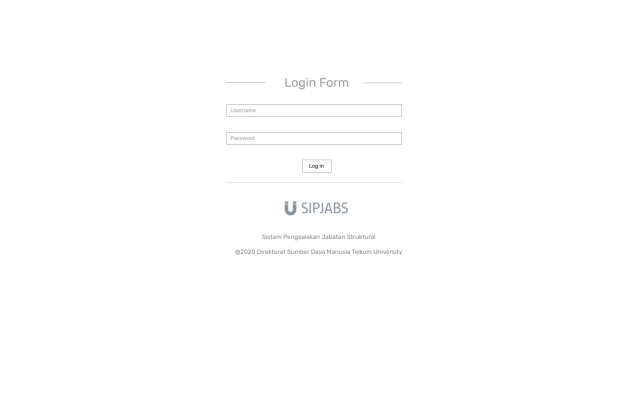
\includegraphics[width=0.6\textwidth, height=60mm]{pics/admin/login.jpg}} 
		& Halaman login merupakan tampilan awal apabila admin membuka aplikasi SiPJabS , admin dapat menginputkan username dan password untuk melakukan login. \\
	
		\hline
		
		2. & \raisebox{-\totalheight}{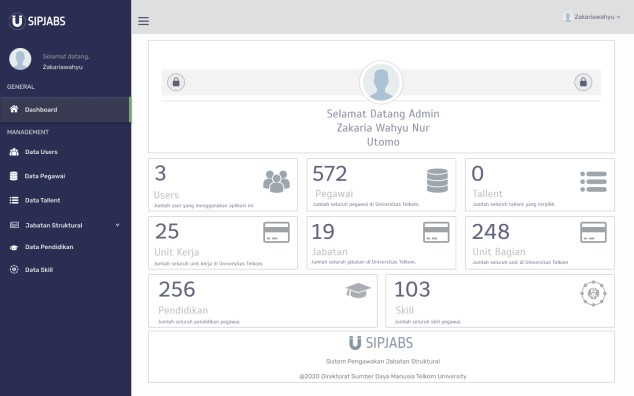
\includegraphics[width=0.6\textwidth, height=60mm]{pics/admin/dashboard.jpg}} 
		& Didalam dashboard admin terdapat jumlah users dari aplikasi SiPJabS, jumlah pegawai di Universitas Telkom, tallent yang sudah dipilih, unit kerja, jabatan, unit bagian, pendidikan dan skill yang dimiliki para pegawai  Universitas Telkom. \\
		\hline

	\end{tabular}
\end{table}


\begin{table}
	\caption{Tabel Perancangan Antar Muka Admin (1)}
	\centering
	\begin{tabular}{ | c | c | p{35mm} |}
		\hline 
		\textbf{No} & \textbf{Gambar} &  \textbf{Keterangan} \\ 
		\hline
		
		3. & \raisebox{-\totalheight}{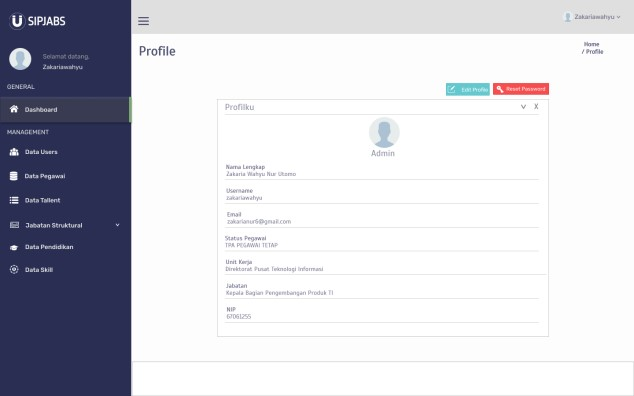
\includegraphics[width=0.6\textwidth, height=60mm]{pics/admin/profile.jpg}} 
		& Halaman profile admin akan menampilkan data profile dari admin tersebut. Kemudian admin juga dapat mengedit profile dan mereset password.  \\
		
		\hline
		
		4. & \raisebox{-\totalheight}{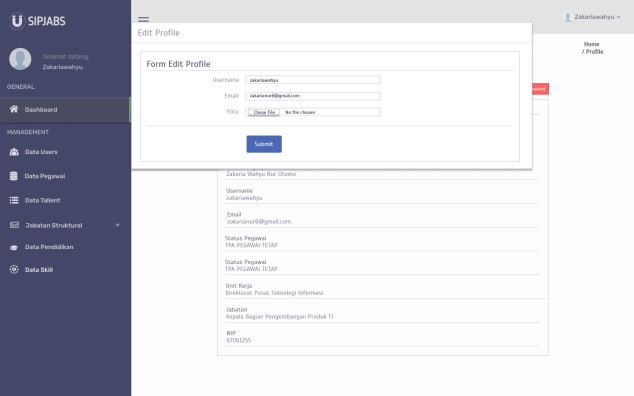
\includegraphics[width=0.6\textwidth, height=60mm]{pics/admin/editprofile.jpg}} 
		& Admin dapat mengubah username, menginputkan email, dan menambahkan foto profile.  \\
		
		\hline
		
		5. & \raisebox{-\totalheight}{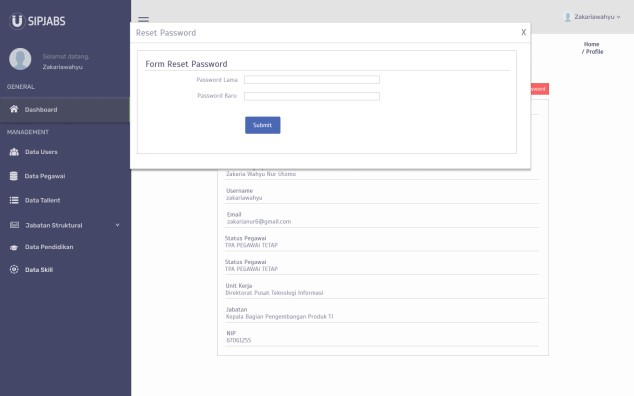
\includegraphics[width=0.6\textwidth, height=60mm]{pics/admin/resetpassword.jpg}} 
		& Admin harus menginputkan password yang lama serta yang baru, setelah itu admin dapat menyimpan. \\
		
		\hline
		
	\end{tabular}
\end{table}

\begin{table}
	\caption{Tabel Perancangan Antar Muka Admin (2)}
	\centering
	\begin{tabular}{ | c | c | p{35mm} |}
		\hline 
		\textbf{No} & \textbf{Gambar} &  \textbf{Keterangan} \\ 
		\hline
		
		
		
		6. & \raisebox{-\totalheight}{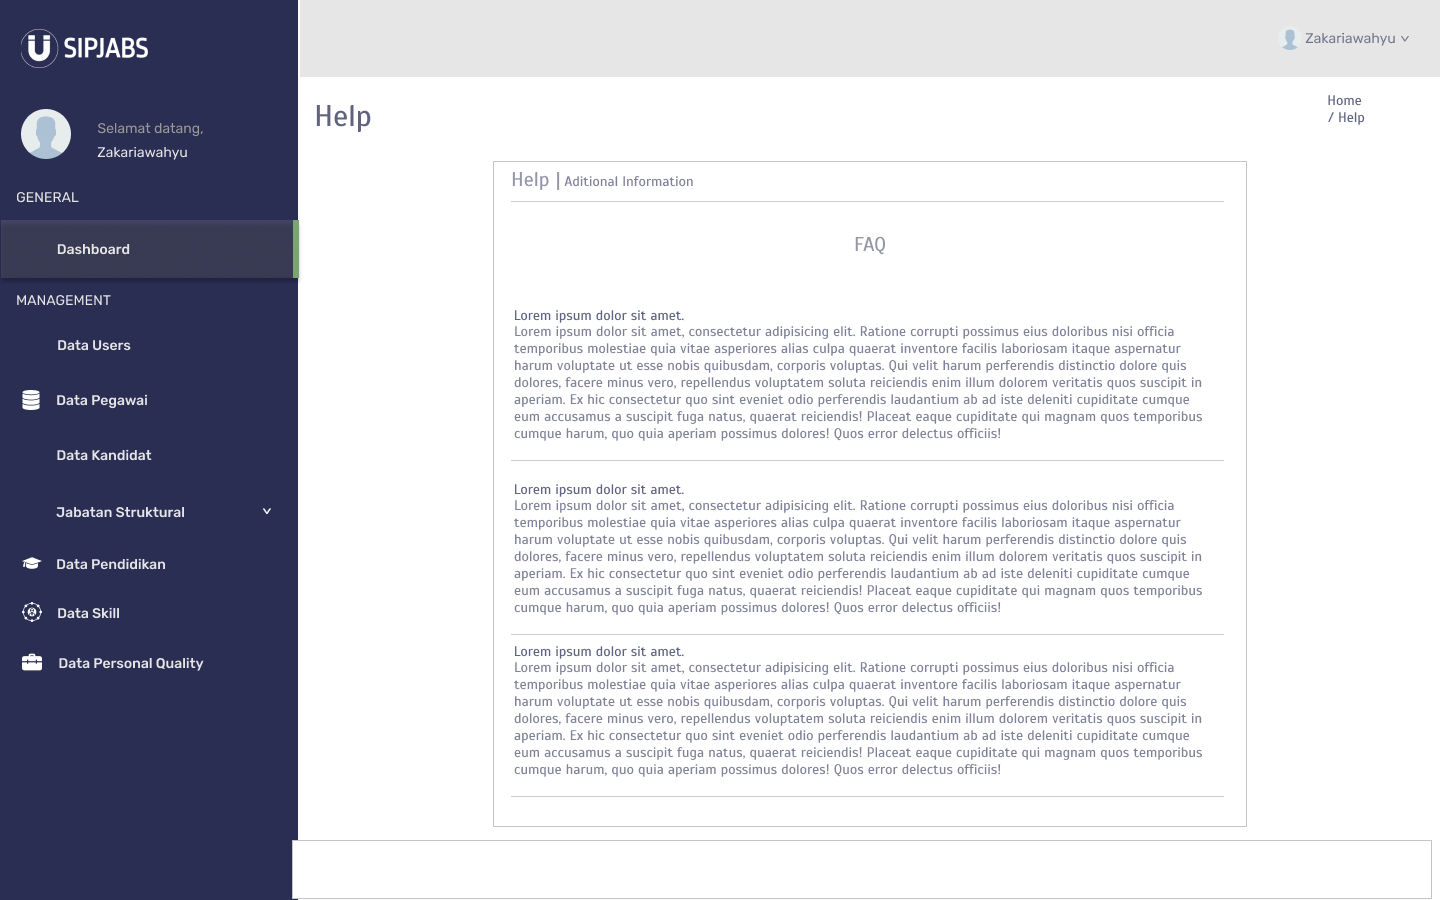
\includegraphics[width=0.6\textwidth, height=60mm]{pics/admin/help.png}} 
		& Halaman help berisi infomasi tentang aplikasi. \\
		
		\hline
		
		7. & \raisebox{-\totalheight}{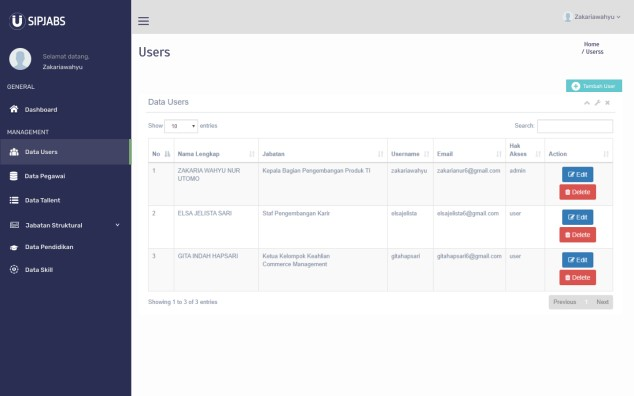
\includegraphics[width=0.6\textwidth, height=60mm]{pics/admin/datausers.jpg}} 
		& Halaman data user akan menampilkan nama-nama yang dapat mengakses aplikasi SiPJabS sebagai admin dan user. \\
		
		\hline
		
		8. & \raisebox{-\totalheight}{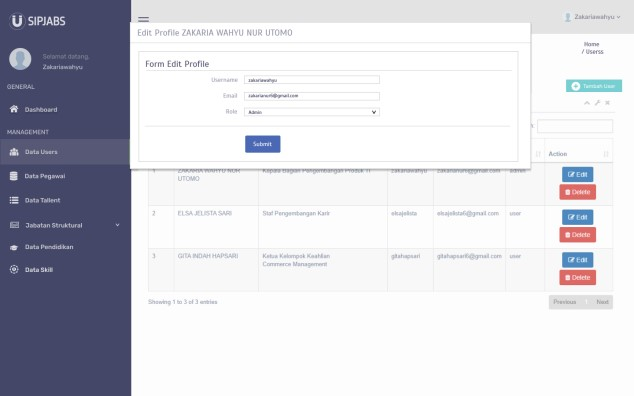
\includegraphics[width=0.6\textwidth, height=60mm]{pics/admin/editdatausers.jpg}} 
		& Pada halaman ini admin dapat mengedit username, email, dan role sebagai admin atau user. \\
		
		\hline
		
	\end{tabular}
\end{table}

\begin{table}
	\caption{Tabel Perancangan Antar Muka Admin (3)}
	\centering
	\begin{tabular}{ | c | c | p{35mm} |}
		\hline 
		\textbf{No} & \textbf{Gambar} &  \textbf{Keterangan} \\ 
		\hline
		
	
		
		9. & \raisebox{-\totalheight}{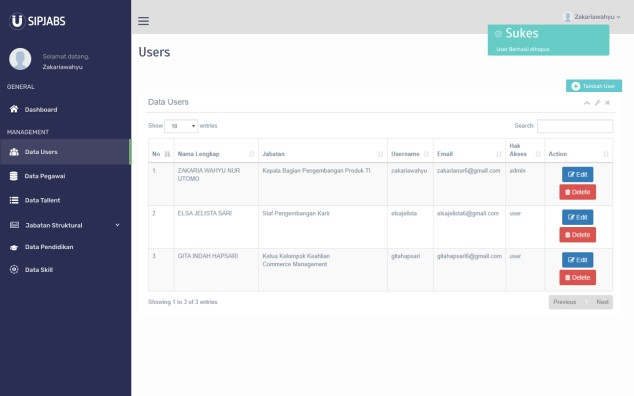
\includegraphics[width=0.6\textwidth, height=60mm]{pics/admin/hapususers.jpg}} 
		&Admin dapat menghapus data user apabila user tersebut sudah tidak bekerja pada bidangnya atau digantikan. \\
		
		\hline
		
		10. & \raisebox{-\totalheight}{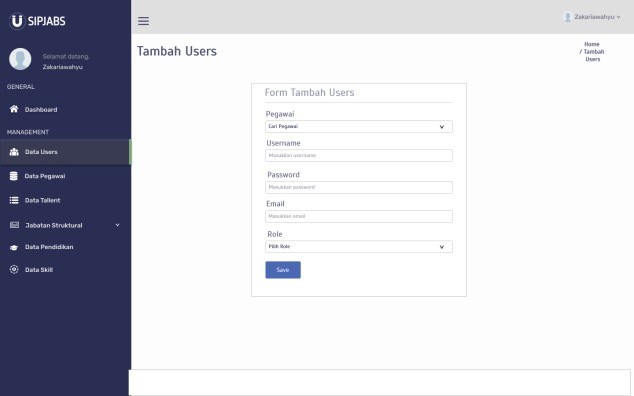
\includegraphics[width=0.6\textwidth, height=60mm]{pics/admin/tambahusers.jpg}} 
		& Admin dapat menambahkan user dengan mengisi form tambah user dan menyimpannya.. \\
		
		\hline
		
		11. & \raisebox{-\totalheight}{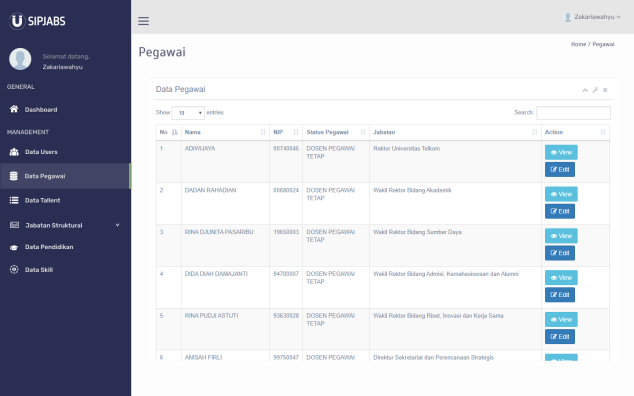
\includegraphics[width=0.6\textwidth, height=60mm]{pics/admin/datapegawai.png}} 
		& Admin dapat melihat daftar data pegawai yang ada di Universitas Telkom secara detail. \\
		
		\hline
		
	\end{tabular}
\end{table}

\begin{table}
	\caption{Tabel Perancangan Antar Muka Admin (4)}
	\centering
	\begin{tabular}{ | c | c | p{35mm} |}
		\hline 
		\textbf{No} & \textbf{Gambar} &  \textbf{Keterangan} \\ 
		\hline
		
		
		
		12. & \raisebox{-\totalheight}{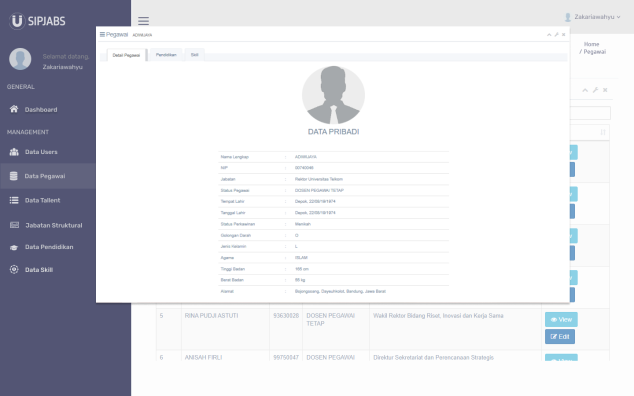
\includegraphics[width=0.6\textwidth, height=60mm]{pics/admin/viewdetailpegawai.png}} 
		&Halaman ini akan menampilkan data pribadi dari pegawai.  \\
		
		\hline
		
		13. & \raisebox{-\totalheight}{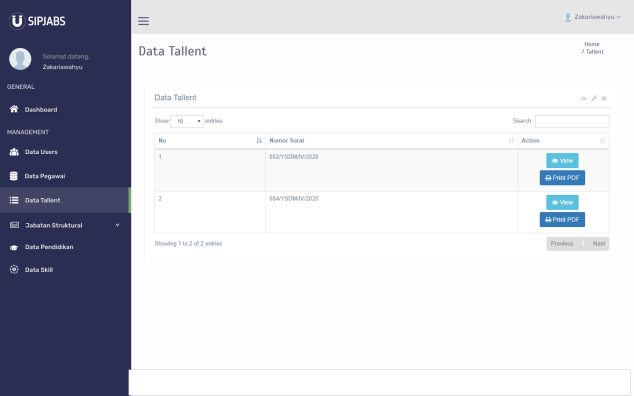
\includegraphics[width=0.6\textwidth, height=60mm]{pics/admin/datatallent.png}} 
		& Halaman ini akan menampilkan data tallent yang sudah di pilih oleh user sesuai dengan job description untuk menggantikan atau mengisi posisi yang kosong. \\
		
		\hline
		
		14. & \raisebox{-\totalheight}{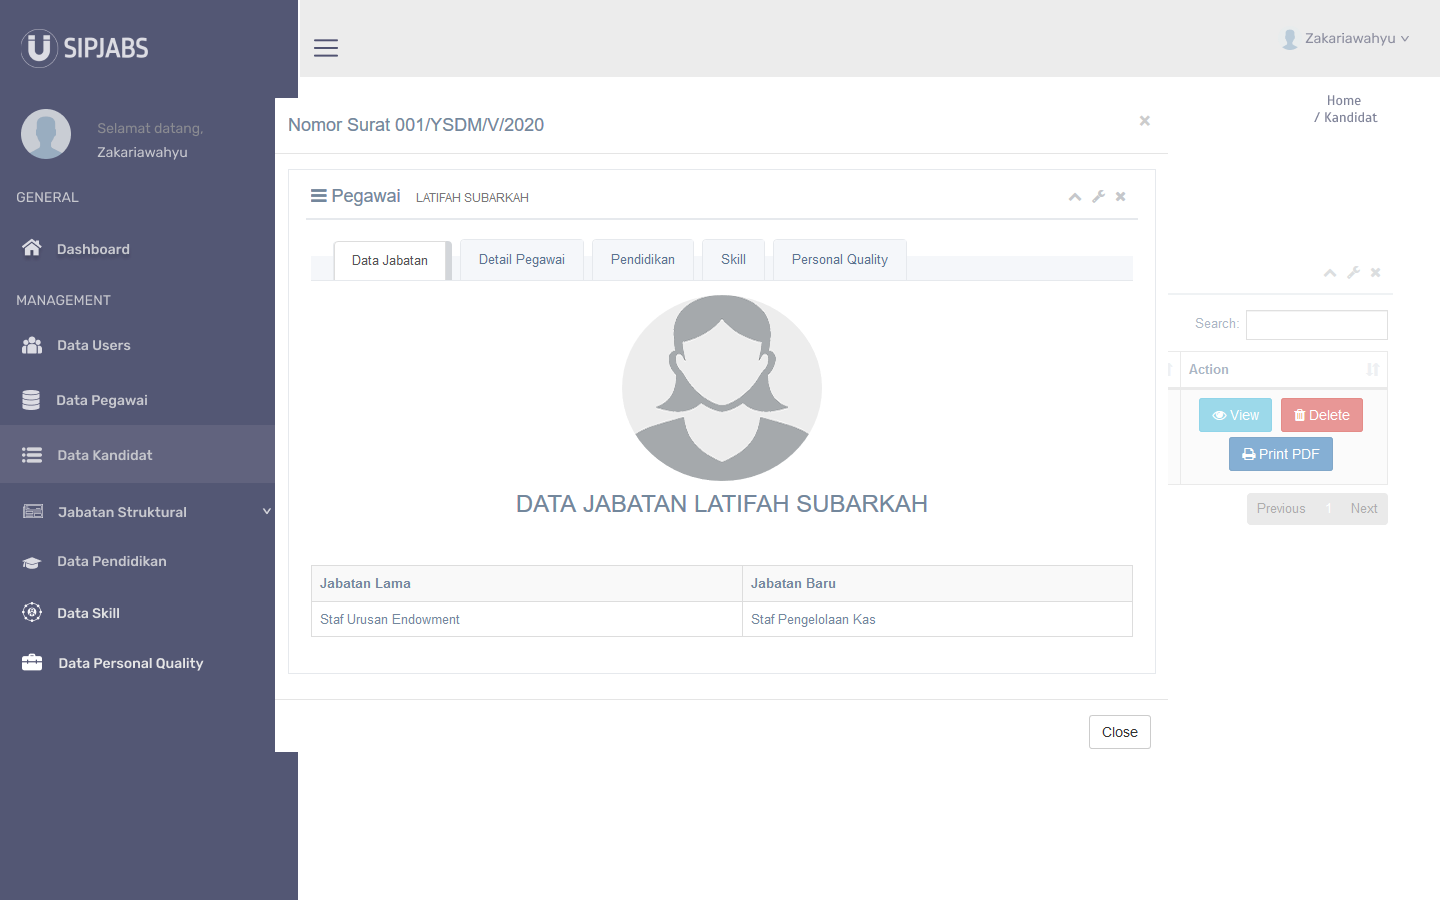
\includegraphics[width=0.6\textwidth, height=60mm]{pics/admin/viewdetailtallent.png}} 
		& Admin dapat melihat data detail tallent yang sudah dipilih. \\
		
		\hline
		
	\end{tabular}
\end{table}

\begin{table}
	\caption{Tabel Perancangan Antar Muka Admin (5)}
	\centering
	\begin{tabular}{ | c | c | p{35mm} |}
		\hline 
		\textbf{No} & \textbf{Gambar} &  \textbf{Keterangan} \\ 
		\hline
		
		
		
		15. & \raisebox{-\totalheight}{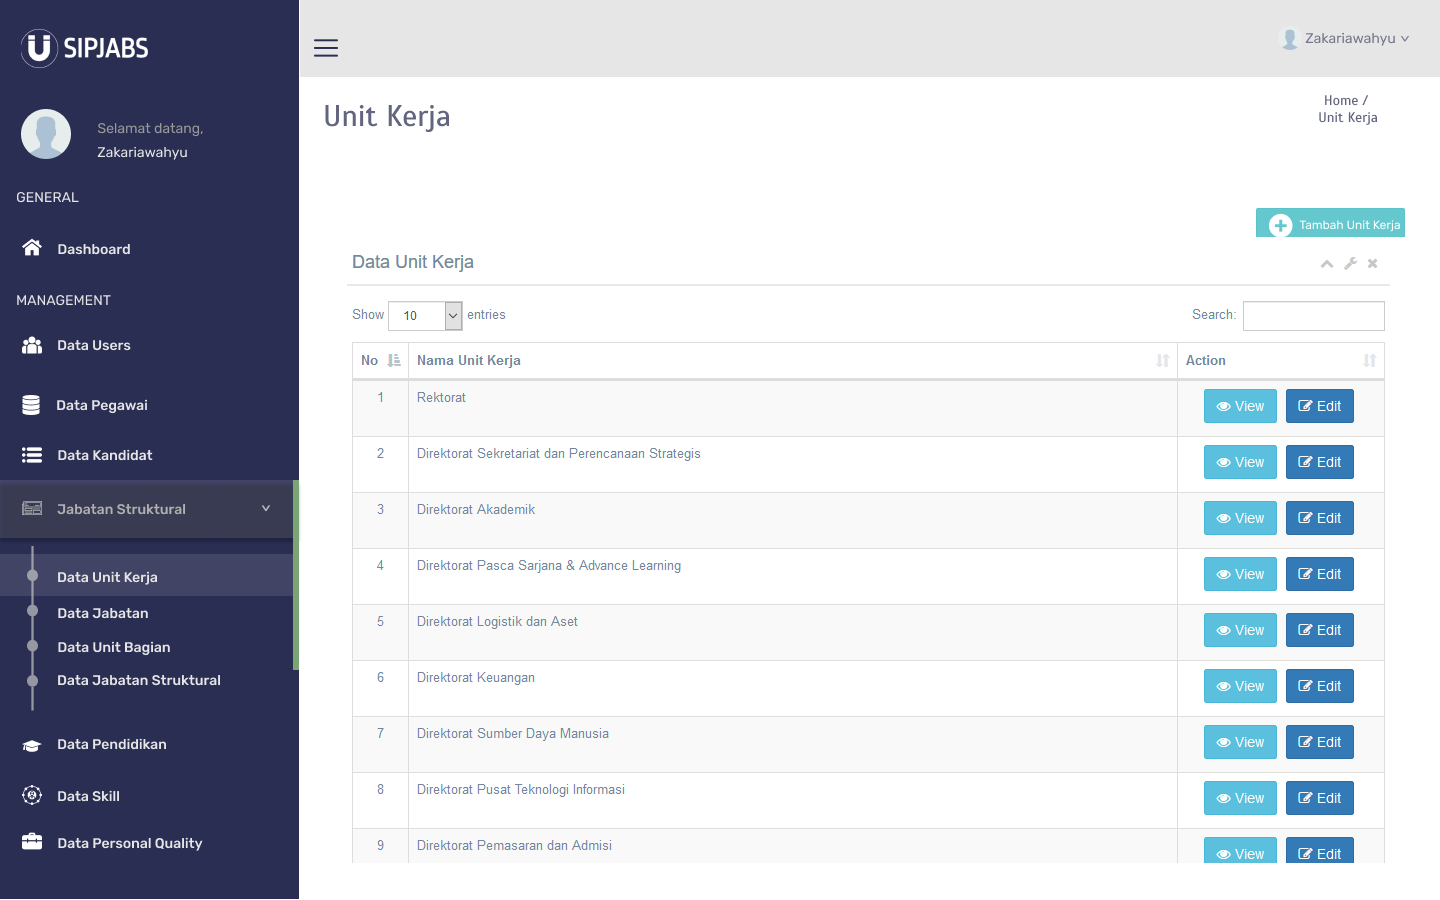
\includegraphics[width=0.6\textwidth, height=60mm]{pics/admin/dataunitkerja.png}} 
		&Halaman ini akan menunjukkan semua unit kerja dimulai dari rektorat hingga fakultas yang ada di Universitas Telkom. \\
		
		\hline
		
		16. & \raisebox{-\totalheight}{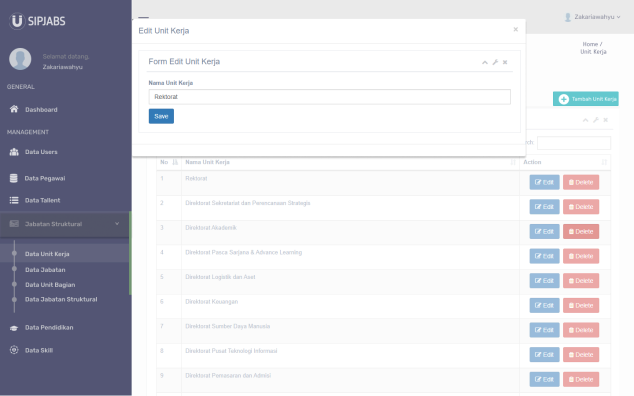
\includegraphics[width=0.6\textwidth, height=60mm]{pics/admin/editunitkerja.png}} 
		& Admin dapat mengedit form unit kerja apabila terdapat kebijakan baru. \\
		
		\hline
		
		17. & \raisebox{-\totalheight}{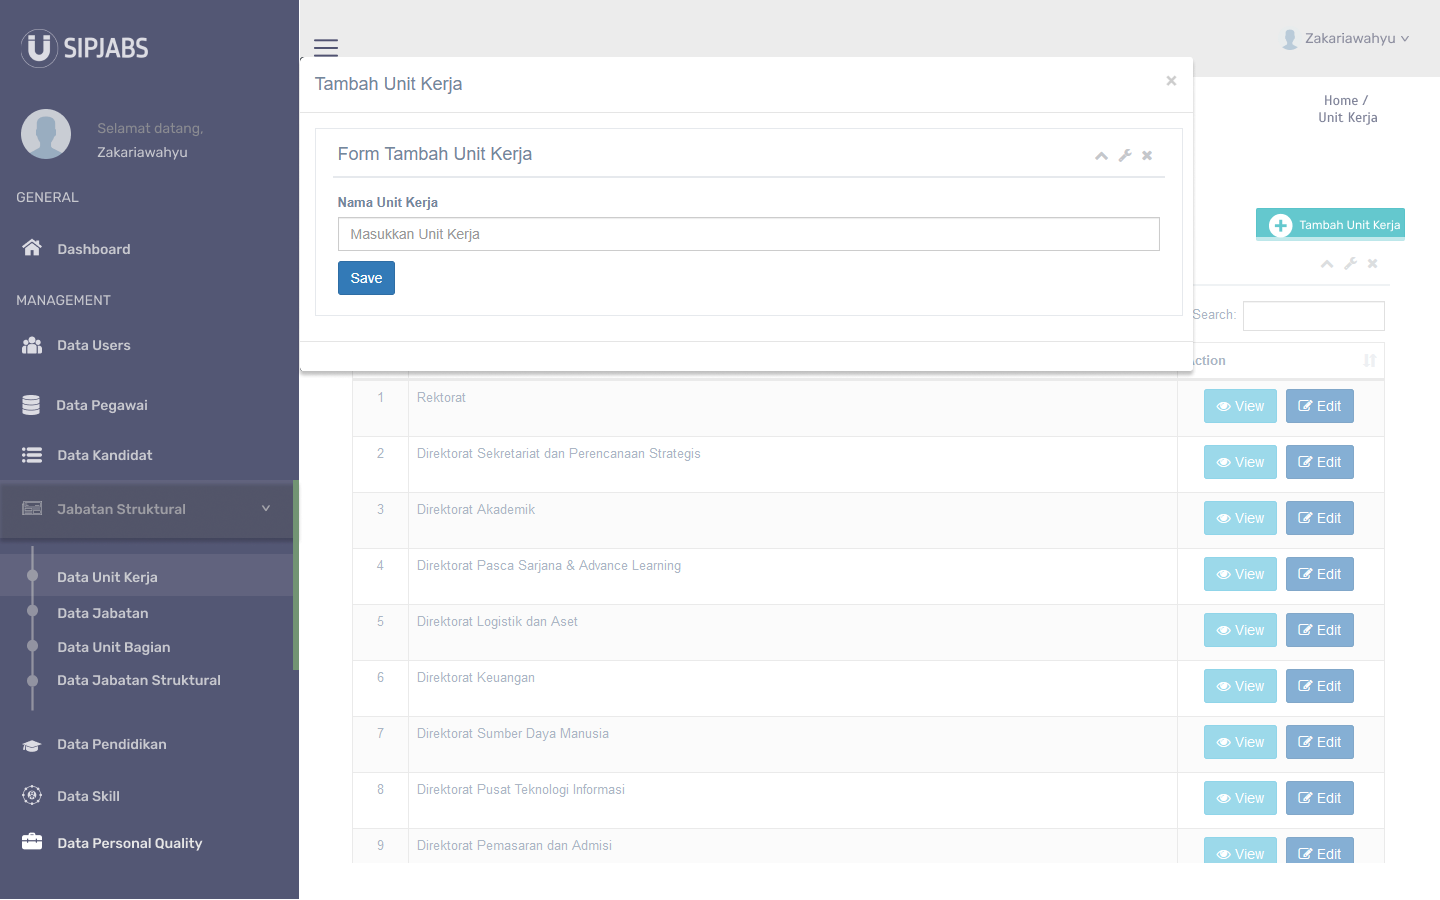
\includegraphics[width=0.6\textwidth, height=60mm]{pics/admin/tambahunitkerja.png}} 
		& Admin dapat menambahkan data unit kerja dengan mengisi form tersebut, namun harus sesuai dengan kebijakan yang telah ditetapkan. \\
		
		\hline
		
	\end{tabular}
\end{table}

\begin{table}
	\caption{Tabel Perancangan Antar Muka Admin (6)}
	\centering
	\begin{tabular}{ | c | c | p{35mm} |}
		\hline 
		\textbf{No} & \textbf{Gambar} &  \textbf{Keterangan} \\ 
		\hline
		
	
		
		18. & \raisebox{-\totalheight}{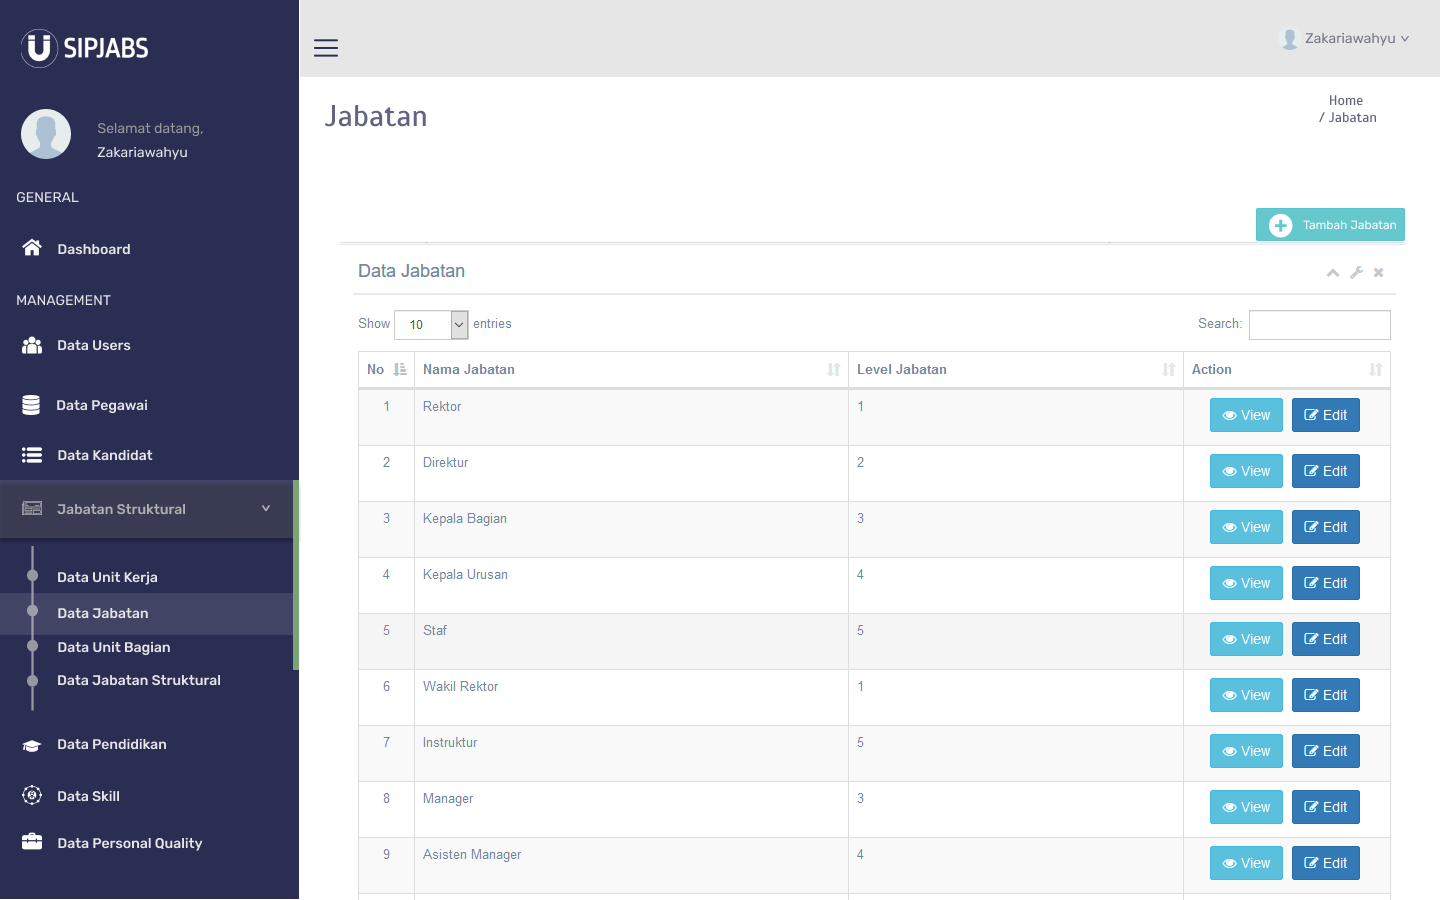
\includegraphics[width=0.6\textwidth, height=60mm]{pics/admin/datajabatan.png}} 
		&Halaman ini akan menampilkan data jabatan yang berada di Universitas Telkom \\
		
		\hline
		
		19. & \raisebox{-\totalheight}{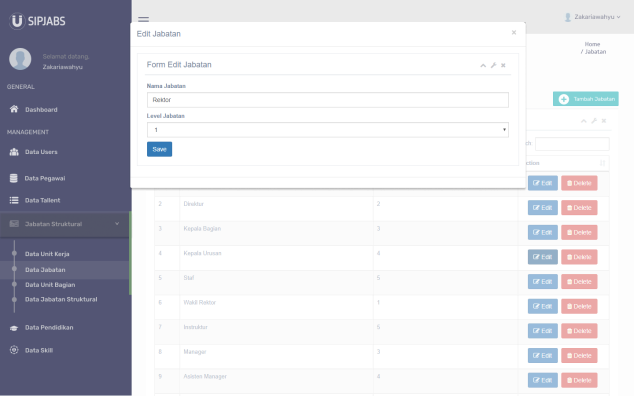
\includegraphics[width=0.6\textwidth, height=60mm]{pics/admin/editjabatan.png}} 
		& Admin dapat mengedit data jabatan sesuai dengan nama jabatan yang sudah ditetapkan. \\
		
		\hline
		
		20. & \raisebox{-\totalheight}{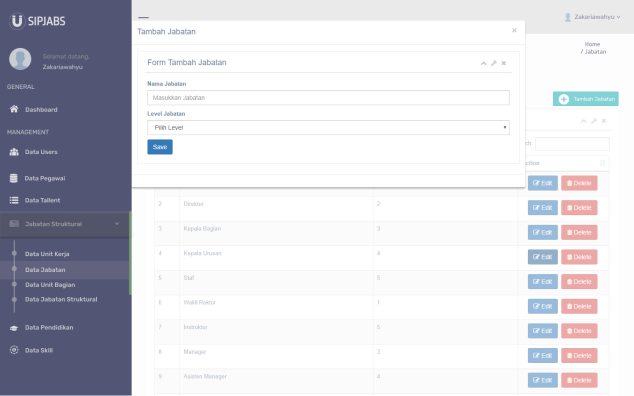
\includegraphics[width=0.6\textwidth, height=60mm]{pics/admin/tambahjabatan.png}} 
		& Admin harus melengkapi form tersebut untuk dapat menambahkan data jabatan yang baru. \\
		
		\hline
		
	\end{tabular}
\end{table}

\begin{table}
	\caption{Tabel Perancangan Antar Muka Admin (7)}
	\centering
	\begin{tabular}{ | c | c | p{35mm} |}
		\hline 
		\textbf{No} & \textbf{Gambar} &  \textbf{Keterangan} \\ 
		\hline
		
		
		
		21. & \raisebox{-\totalheight}{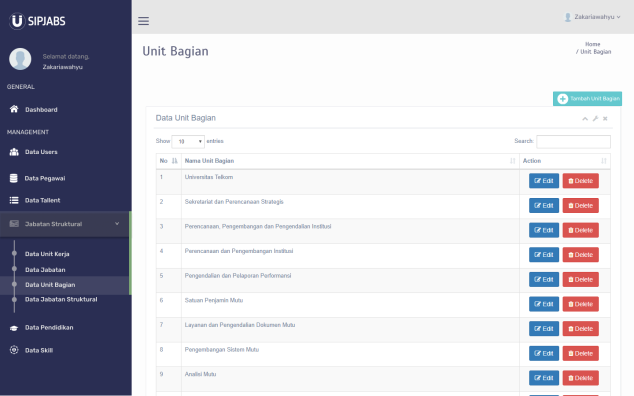
\includegraphics[width=0.6\textwidth, height=60mm]{pics/admin/dataunitbagian.png}} 
		&Halaman ini akan menampilkan satuan kerja yang terdapat di Universitas Telkom.  \\
		
		\hline
		
		22. & \raisebox{-\totalheight}{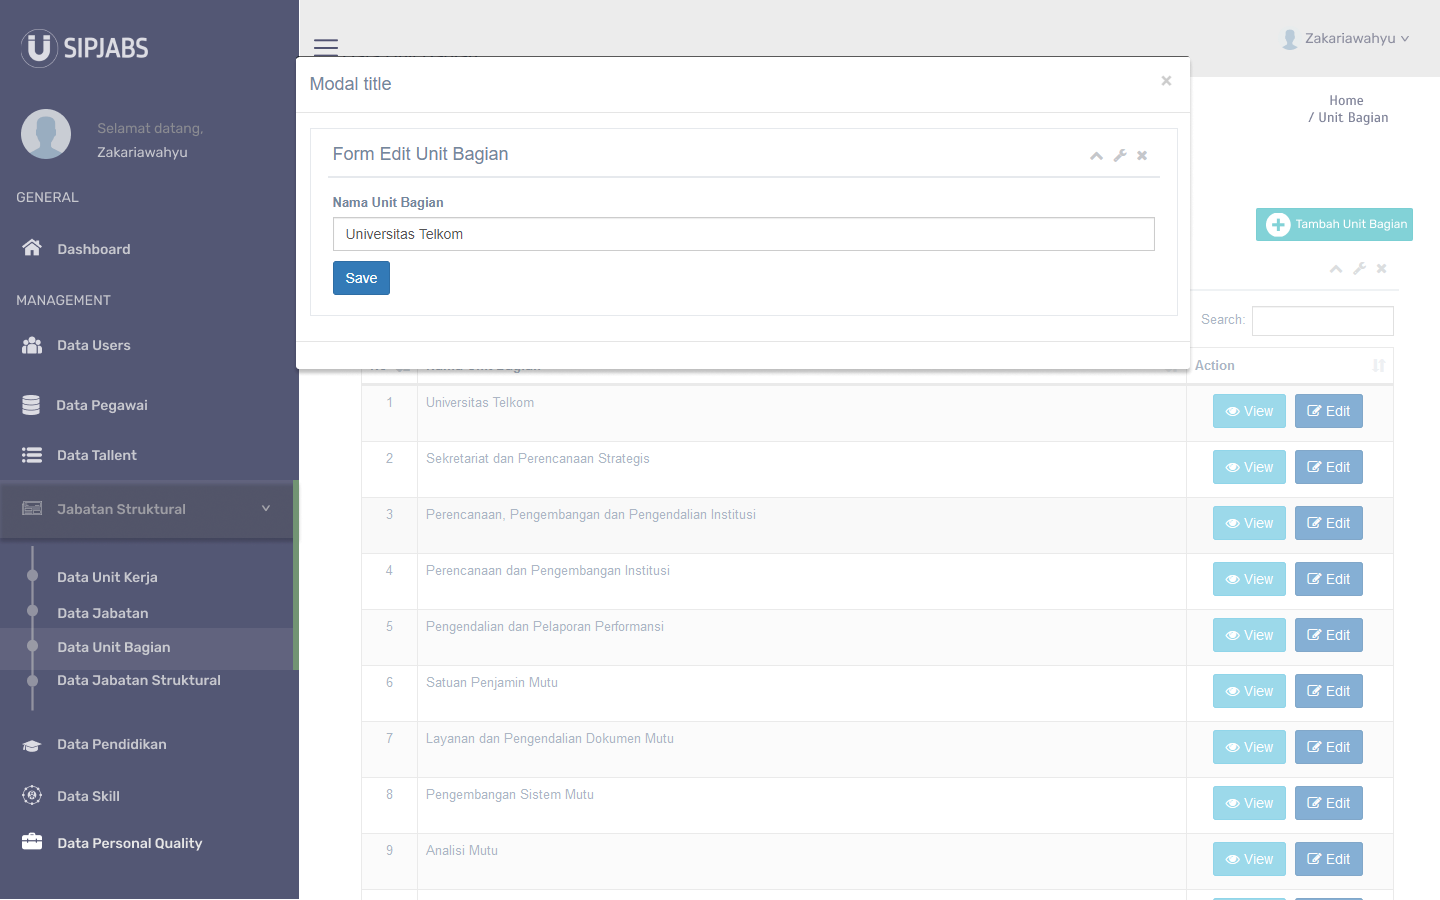
\includegraphics[width=0.6\textwidth, height=60mm]{pics/admin/editunitbagian.png}} 
		& Admin dapat mengedit data unit bagian apabila ada perubahan yang sudah ditetapkan.\\
		
		\hline
		
		23. & \raisebox{-\totalheight}{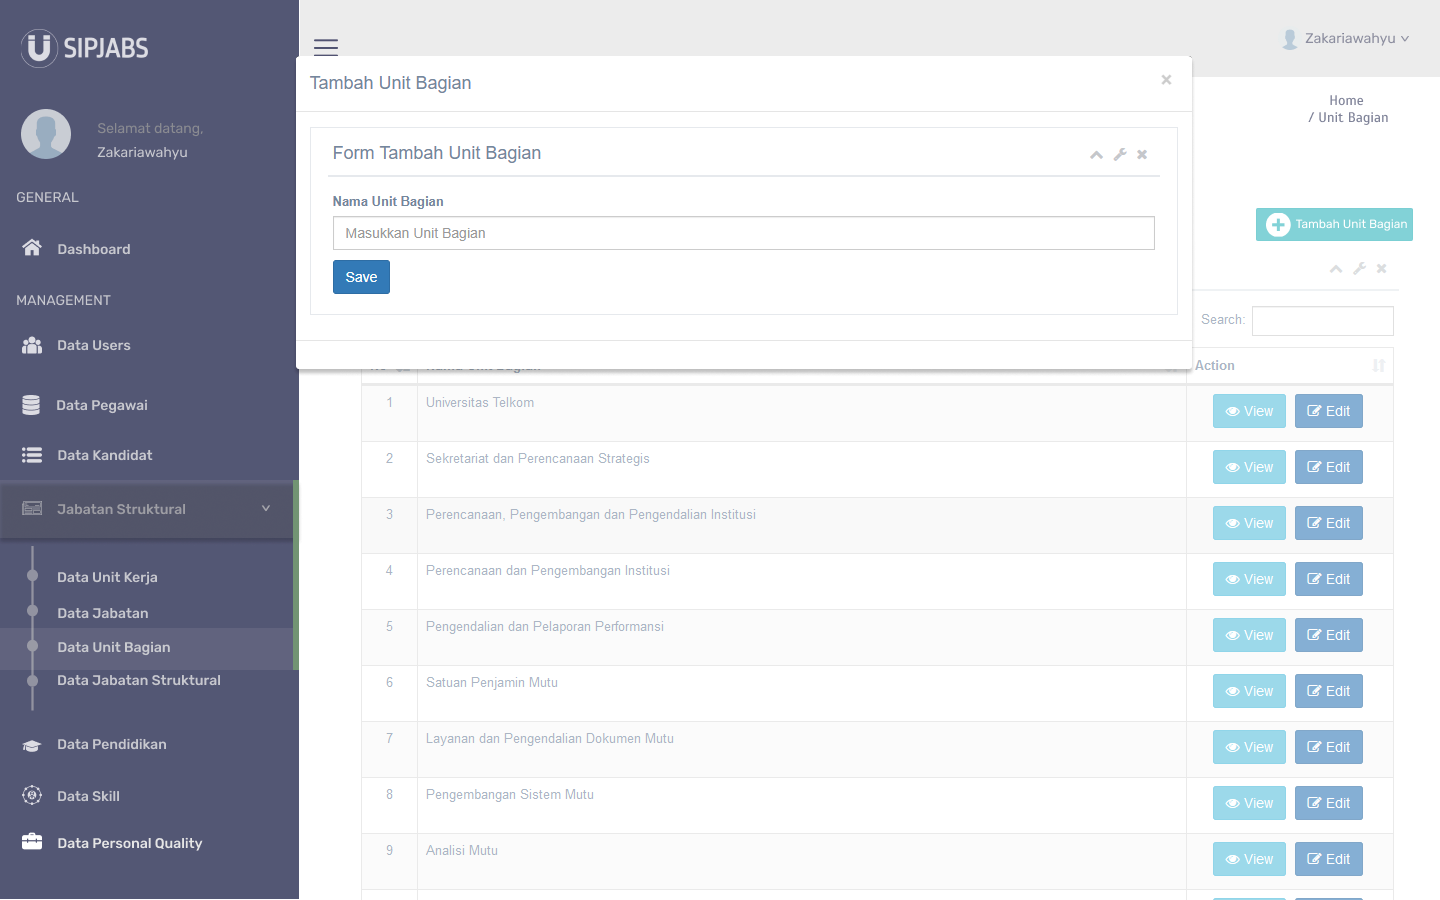
\includegraphics[width=0.6\textwidth, height=60mm]{pics/admin/tambahunitbagian.png}} 
		& Admin harus menginputkan  nama unit bagian  tersebut untuk dapat menambahkan data data unit bagian yang baru. \\
		
		\hline
		
	\end{tabular}
\end{table}

\begin{table}
	\caption{Tabel Perancangan Antar Muka Admin (8)}
	\centering
	\begin{tabular}{ | c | c | p{35mm} |}
		\hline 
		\textbf{No} & \textbf{Gambar} &  \textbf{Keterangan} \\ 
		\hline
		
		
		
		24. & \raisebox{-\totalheight}{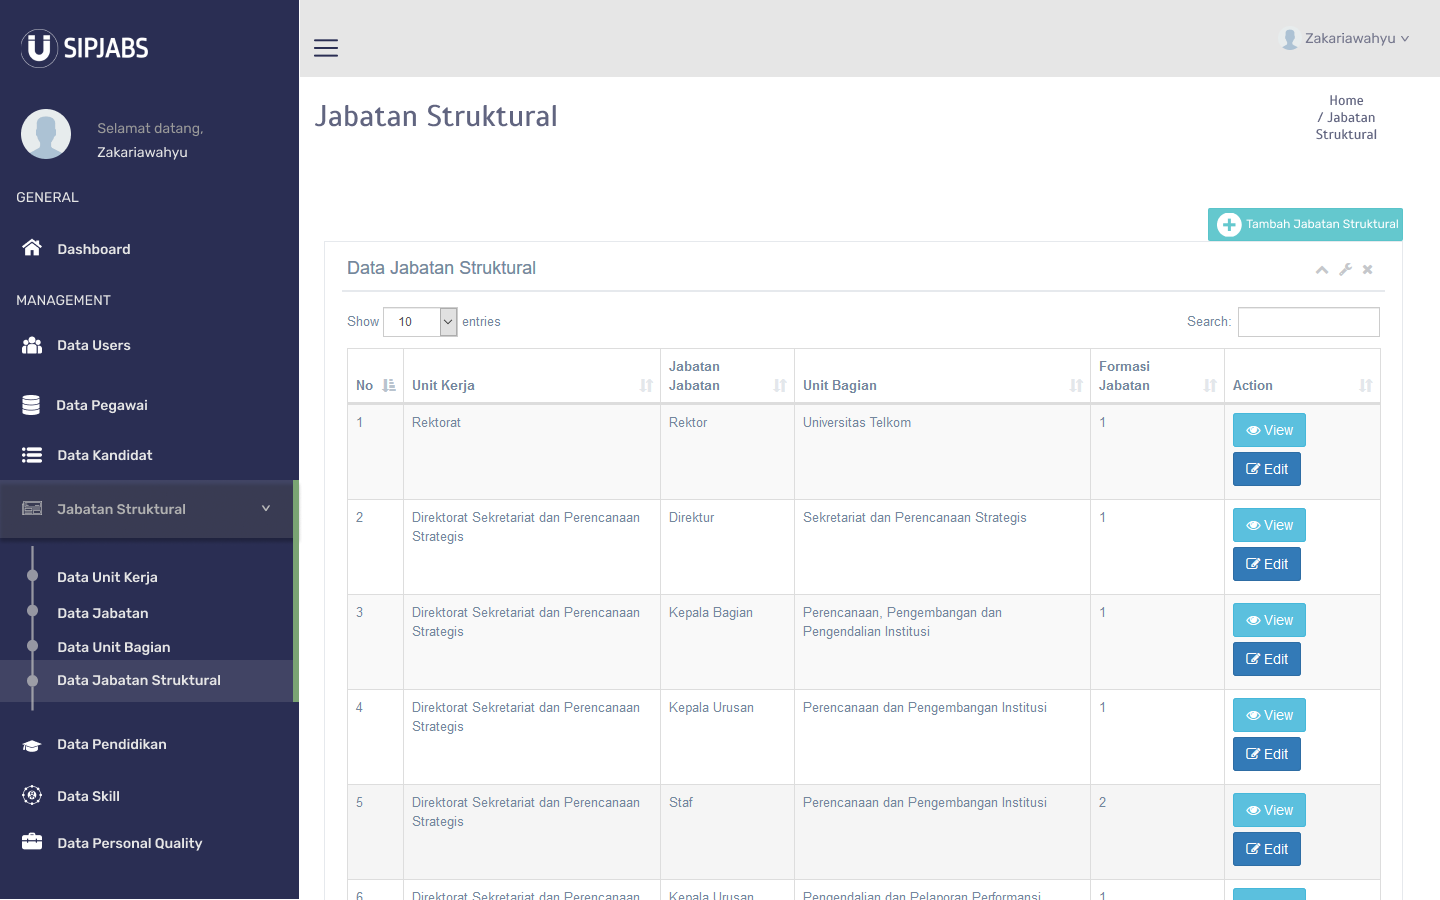
\includegraphics[width=0.6\textwidth, height=60mm]{pics/admin/datajabstruk.png}} 
		&Halaman ini menampilkan jabatan yang secara tegas ada di Universitas Telkom.  \\
		
		\hline
		
		25. & \raisebox{-\totalheight}{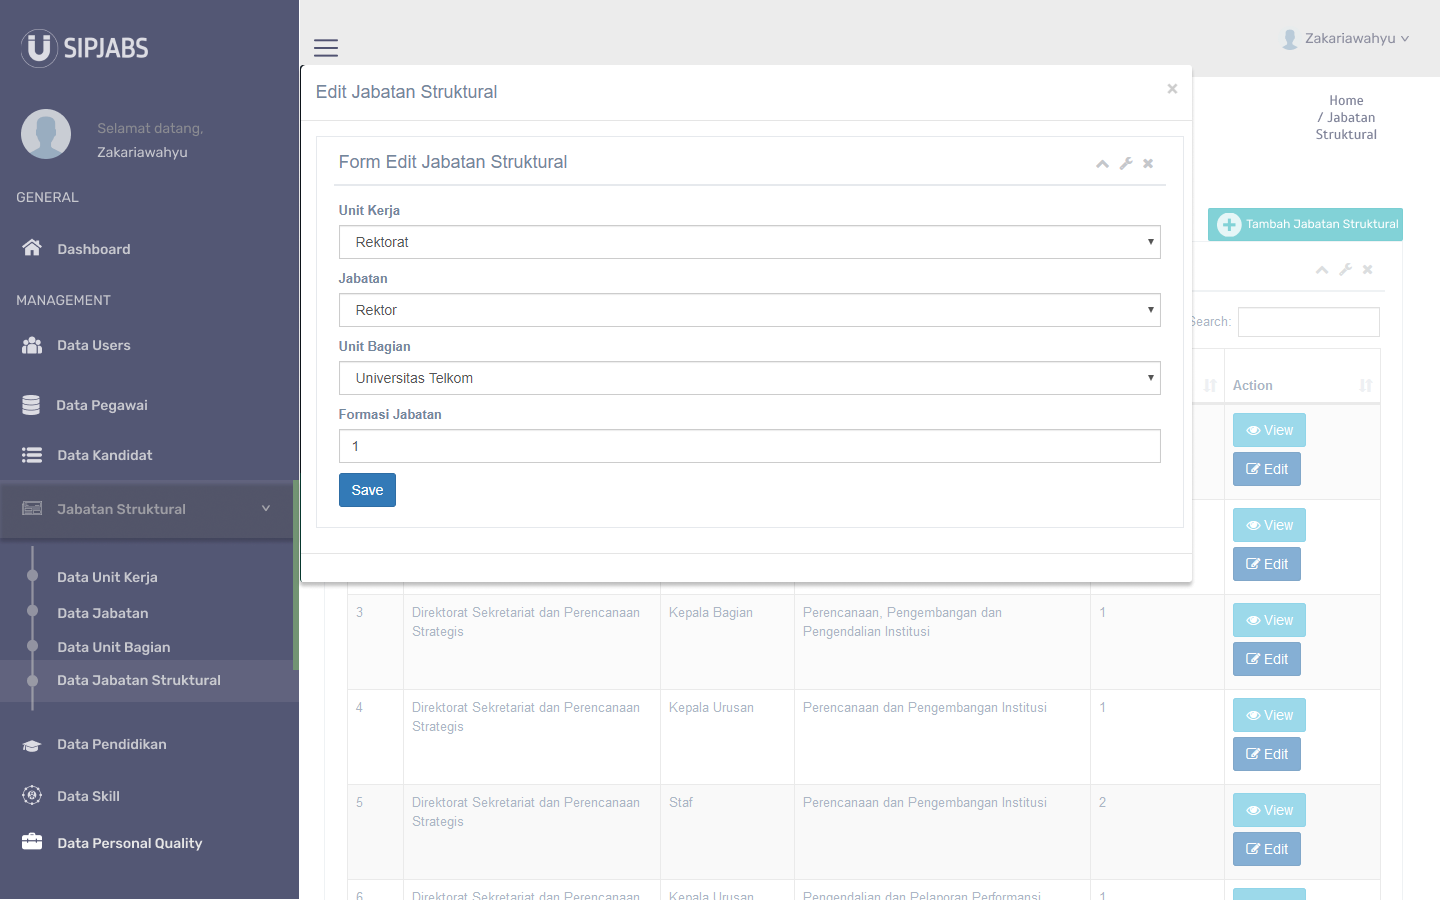
\includegraphics[width=0.6\textwidth, height=60mm]{pics/admin/editjabstruk.png}} 
		& Admin dapat mengedit data dan harus mengisi form sesuai dengan ketetapan.\\
		
		\hline
		
		26. & \raisebox{-\totalheight}{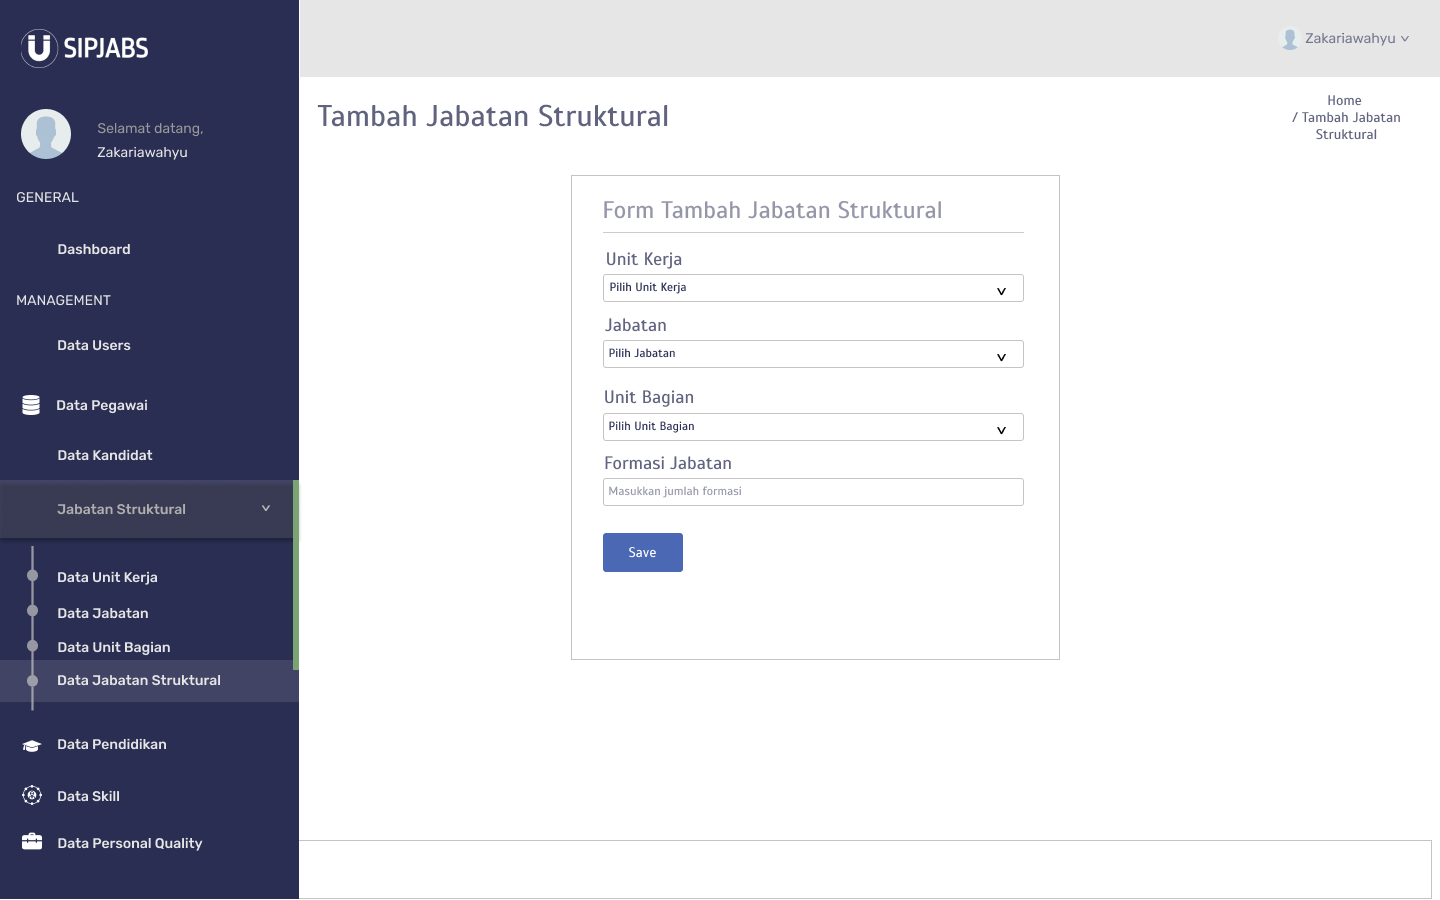
\includegraphics[width=0.6\textwidth, height=60mm]{pics/admin/tambahjabstruk.png}} 
		& Admin harus melengkapi form untuk dapat menambahkan data jabatan struktural baru yang sudah ditetapkan. \\
		
		\hline
		
	\end{tabular}
\end{table}

\begin{table}
	\caption{Tabel Perancangan Antar Muka Admin (9)}
	\centering
	\begin{tabular}{ | c | c | p{35mm} |}
		\hline 
		\textbf{No} & \textbf{Gambar} &  \textbf{Keterangan} \\ 
		\hline
		
		
		
		27. & \raisebox{-\totalheight}{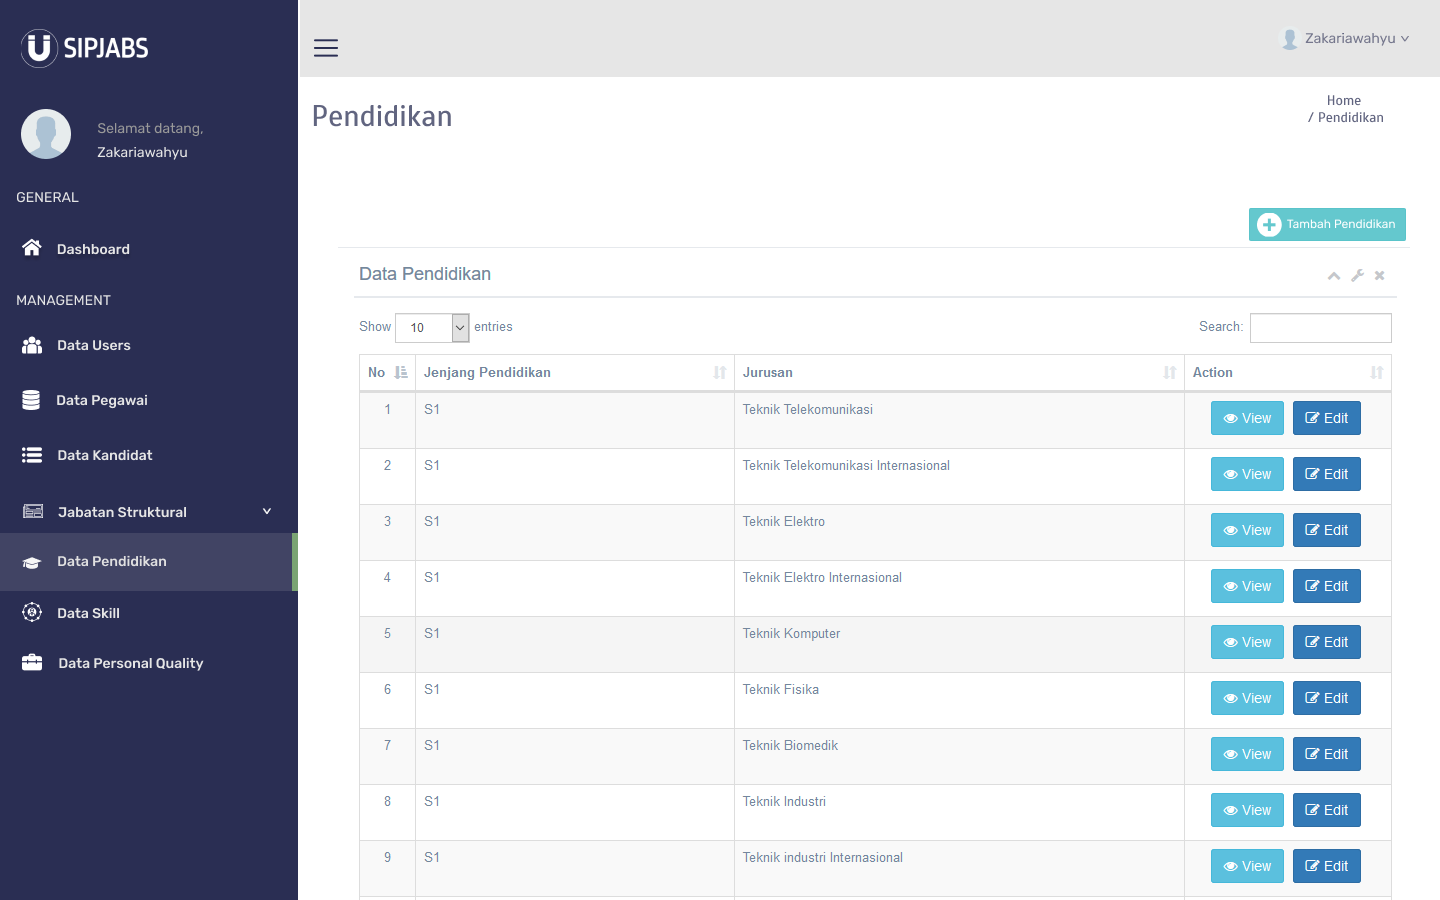
\includegraphics[width=0.6\textwidth, height=60mm]{pics/admin/datapendidikan.png}} 
		&Halaman ini akan menampilkan data pendidikan yang dimiliki pegawai Universitas Telkom.  \\
		
		\hline
		
		28. & \raisebox{-\totalheight}{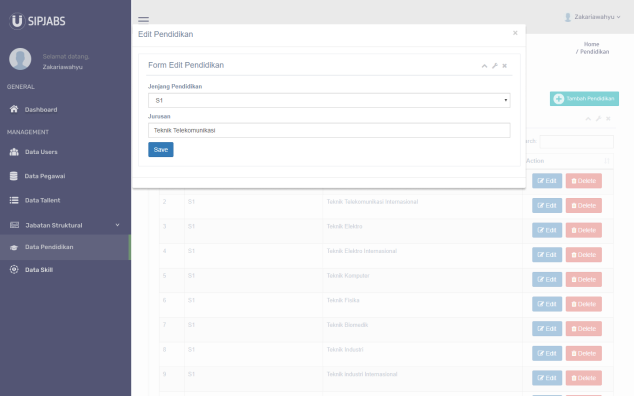
\includegraphics[width=0.6\textwidth, height=60mm]{pics/admin/editpendidikan.png}} 
		& Apabila ingin mengedit maka admin harus menginputkan jenjang pendidikan serta jurusan. \\
		
		\hline
		
		29. & \raisebox{-\totalheight}{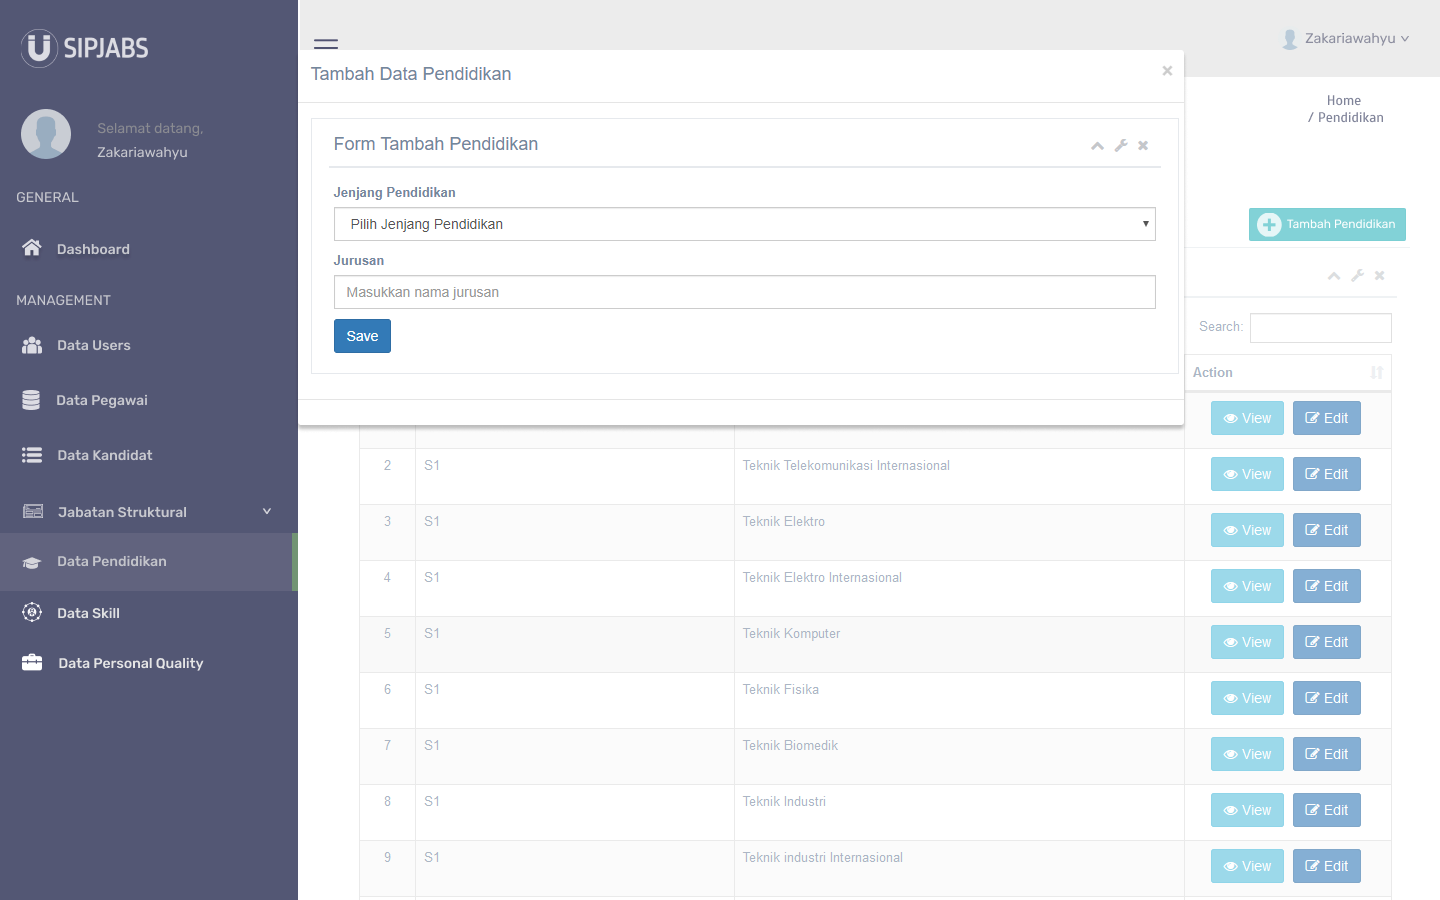
\includegraphics[width=0.6\textwidth, height=60mm]{pics/admin/tambahpendidikan.png}} 
		& Admin dapat menambahkan data pendidikan apabila belum ada data pendidikan yang dimiliki pegawai belum terinput. \\
		
		\hline
		
	\end{tabular}
\end{table}

\begin{table}
	\caption{Tabel Perancangan Antar Muka Admin (10)}
	\centering
	\begin{tabular}{ | c | c | p{35mm} |}
		\hline 
		\textbf{No} & \textbf{Gambar} &  \textbf{Keterangan} \\ 
		\hline
		
		
		
		30. & \raisebox{-\totalheight}{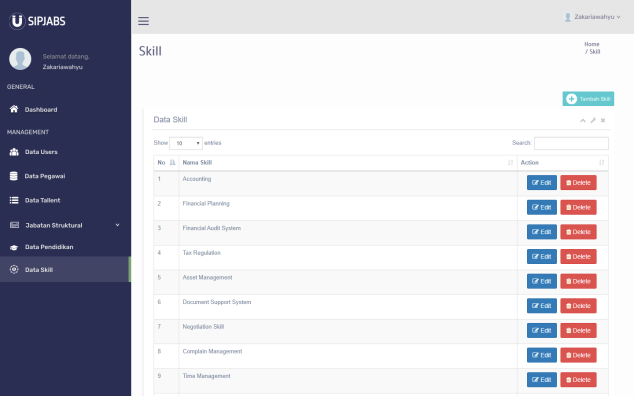
\includegraphics[width=0.6\textwidth, height=60mm]{pics/admin/dataskill.png}} 
		&Halaman ini akan menampilkan skill yang dimiliki pegawai Universitas Telkom untuk menunjang pekerjaan.  \\
		
		\hline
		
		31. & \raisebox{-\totalheight}{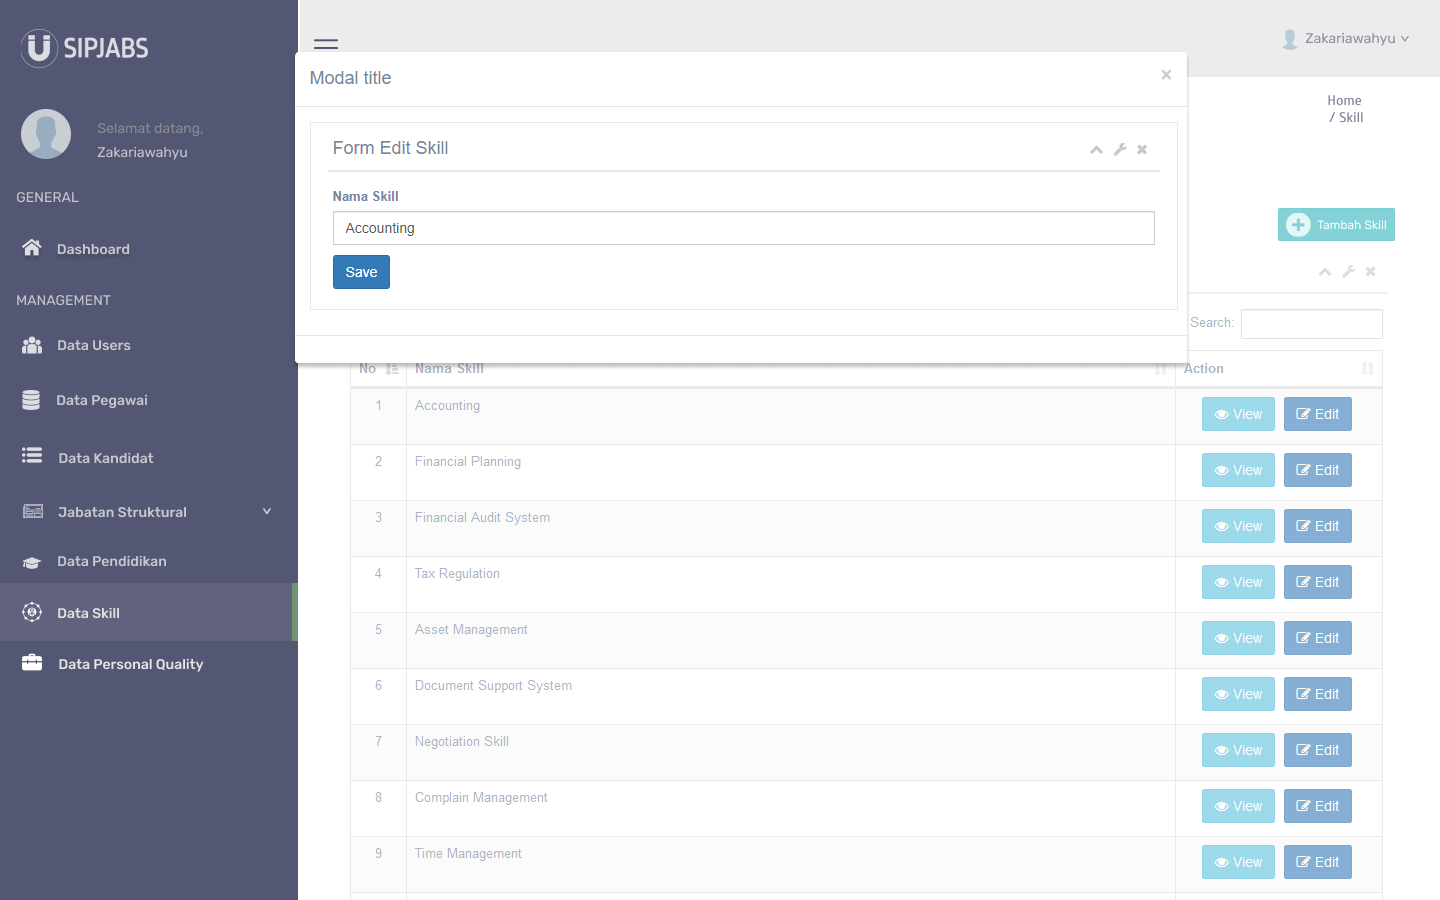
\includegraphics[width=0.6\textwidth, height=60mm]{pics/admin/editskill.png}} 
		& Admin dapat mengedit data skill. \\
		
		\hline
		
		32. & \raisebox{-\totalheight}{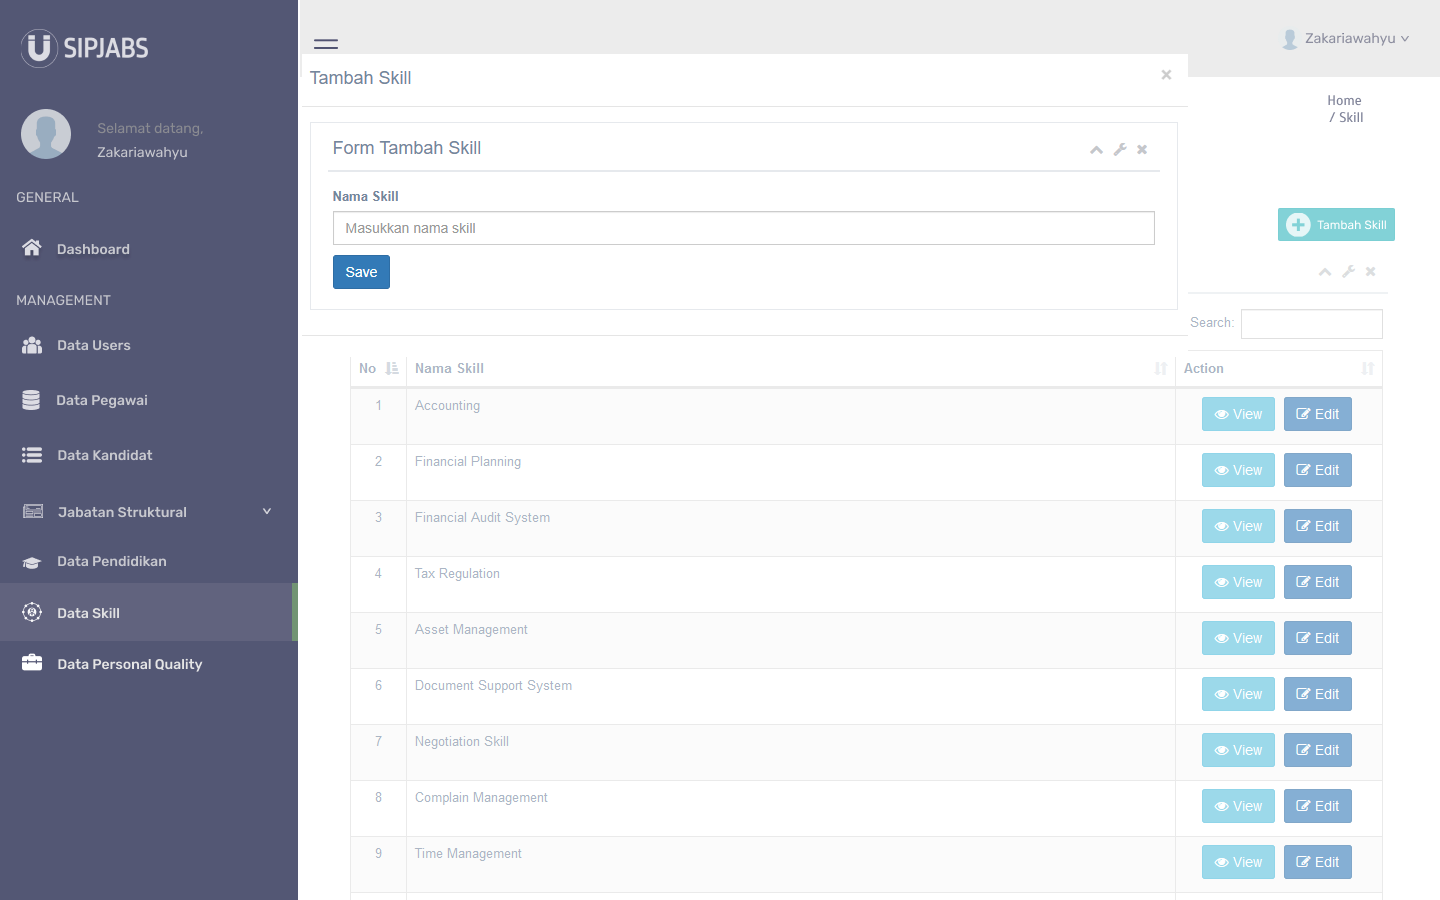
\includegraphics[width=0.6\textwidth, height=60mm]{pics/admin/tambahskill.png}} 
		& Admin dapat menambahkan data skill baru apabila terdapat data skill yang belum diinputkan.  \\
		
		\hline
		
	\end{tabular}
\end{table}

\subsubsection{Perancangan Antar Muka User}

\begin{table}
	\caption{Tabel Perancangan Antar Muka User}
	\centering
	\begin{tabular}{ | c | c | p{35mm} |}
		\hline 
		\textbf{No} & \textbf{Gambar} &  \textbf{Keterangan} \\ 
		\hline
		
		1. & \raisebox{-\totalheight}{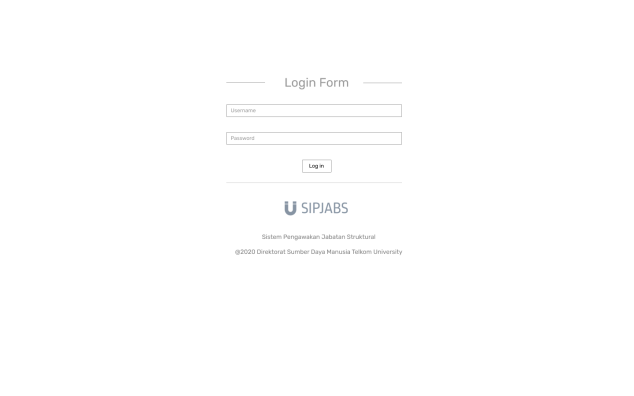
\includegraphics[width=0.6\textwidth, height=60mm]{pics/user/login.png}} 
		& Halaman login merupakan tampilan awal apabila user membuka aplikasi SiPJabS ,user dapat menginputkan username dan password untuk melakukan login.  \\
		
		\hline
		
		2. & \raisebox{-\totalheight}{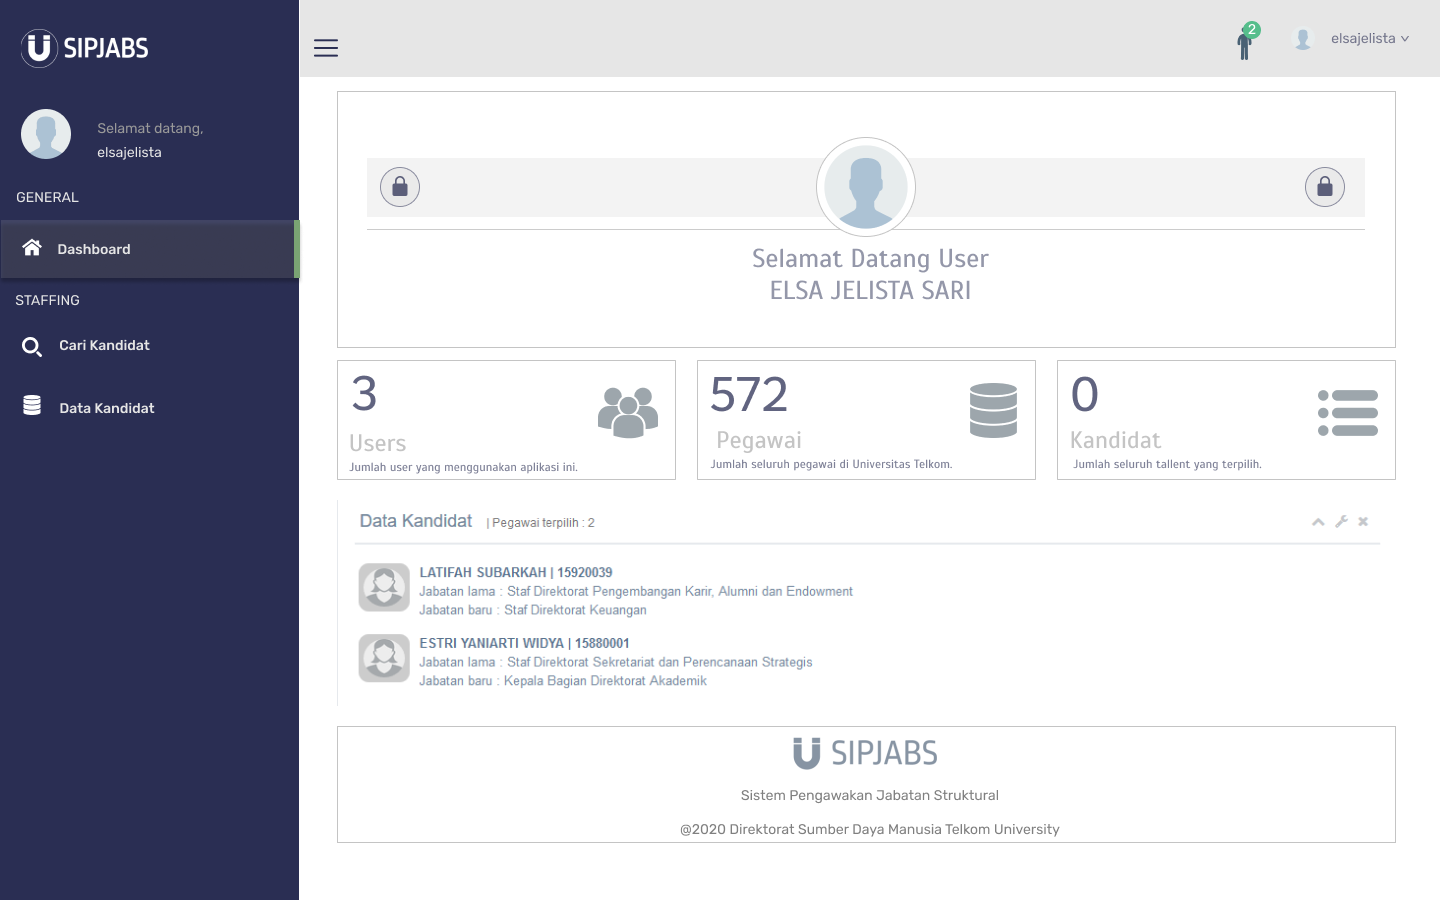
\includegraphics[width=0.6\textwidth, height=60mm]{pics/user/dashboard.png}} 
		& Halaman ini akan menampilkan jumlah user yang dapat mengakses aplikasi SiPJabS, jumlah pegawai yang ada di Universitas Telkom serta jumlah tallent yang sudah dipilih.  \\
		
		\hline
		
		3. & \raisebox{-\totalheight}{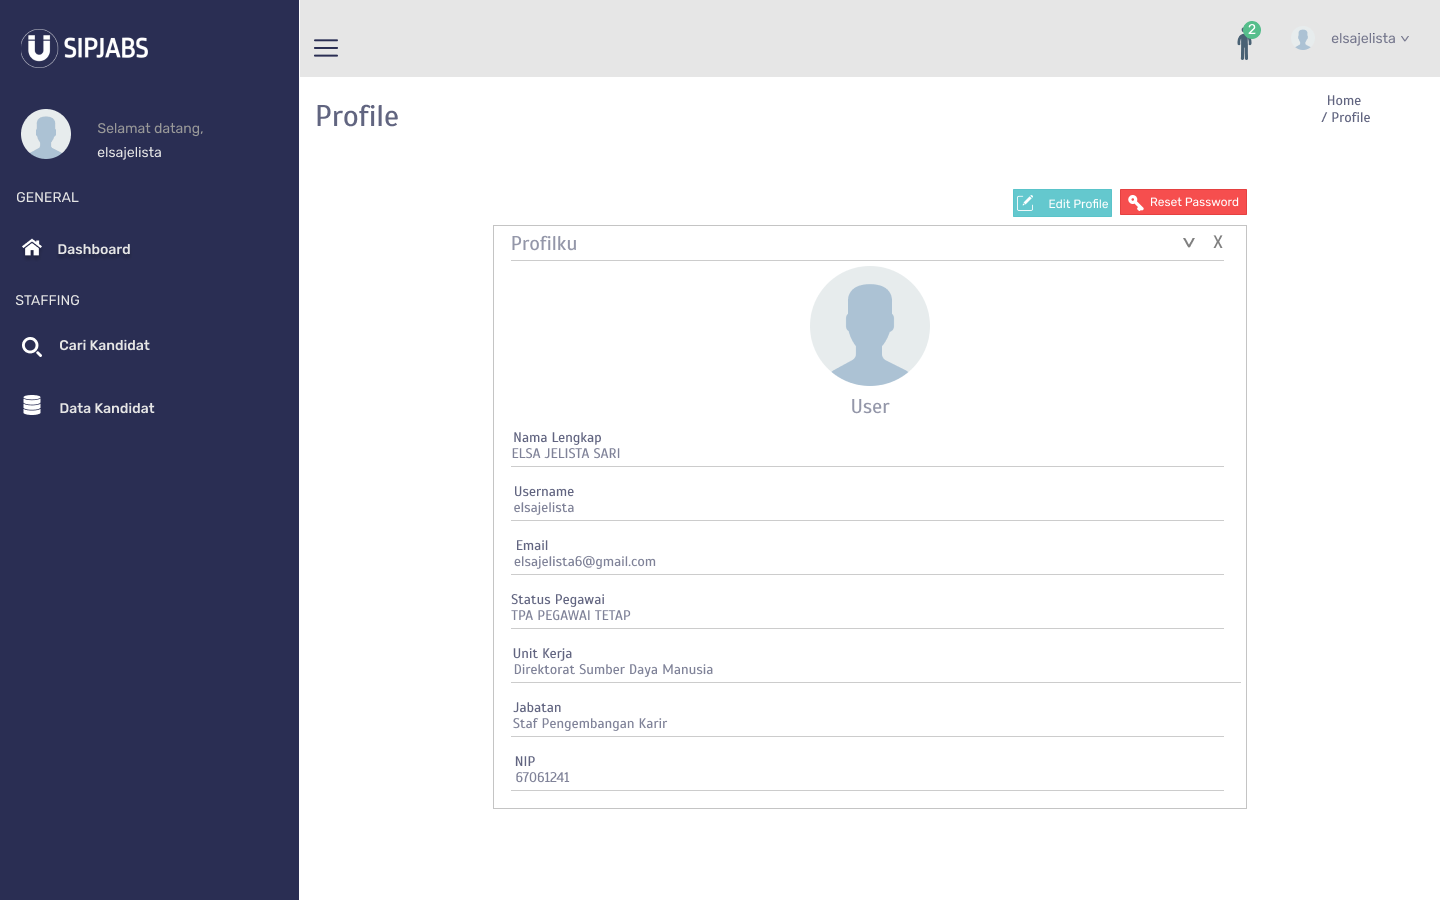
\includegraphics[width=0.6\textwidth, height=60mm]{pics/user/profile.png}} 
		& Halaman profile user akan menampilkan data nama lengkap, username, email, status pegawai, unit kerja, jabatan, serta NIP dari user tersebut. Kemudian user juga dapat mengedit profile dan mereset password.\\
		
		\hline
		
		
	\end{tabular}
\end{table}

\begin{table}
	\caption{Tabel Perancangan Antar Muka User (1)}
	\centering
	\begin{tabular}{ | c | c | p{35mm} |}
		\hline 
		\textbf{No} & \textbf{Gambar} &  \textbf{Keterangan} \\ 
		\hline
		
		4. & \raisebox{-\totalheight}{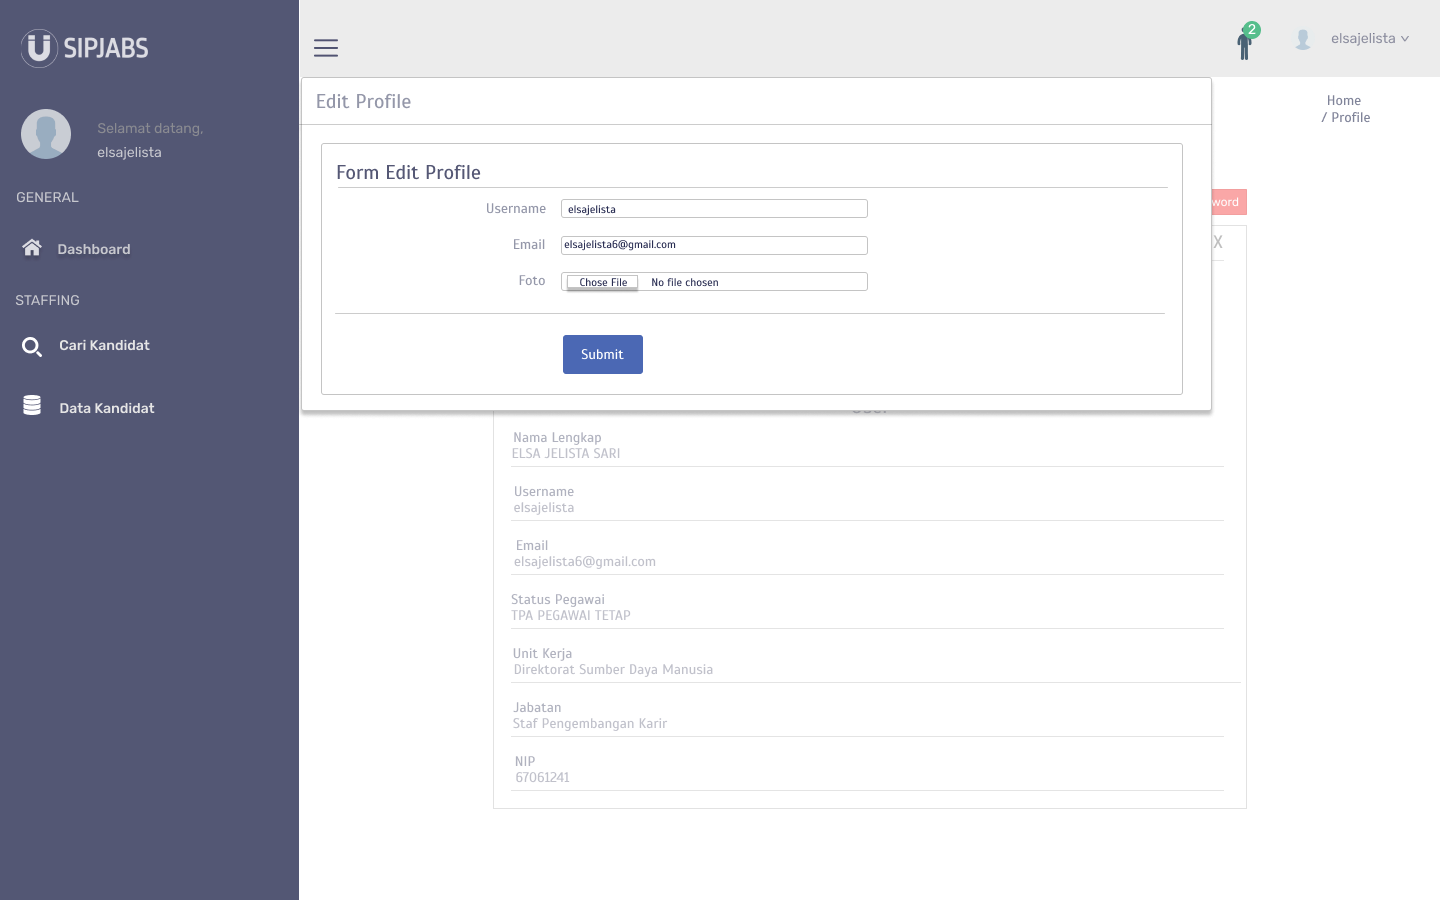
\includegraphics[width=0.6\textwidth, height=60mm]{pics/user/editprofile.png}} 
		& User dapat mengubah username, menginputkan email, dan menambahkan foto profile  \\
		
		\hline
		
		5. & \raisebox{-\totalheight}{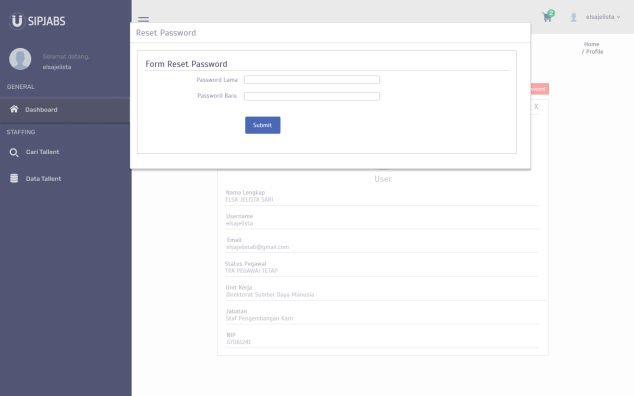
\includegraphics[width=0.6\textwidth, height=60mm]{pics/user/resetpassword.png}} 
		& User harus menginputkan password yang lama serta yang baru, setelah itu user dapat menyimpan.  \\
		
		\hline
		
		6. & \raisebox{-\totalheight}{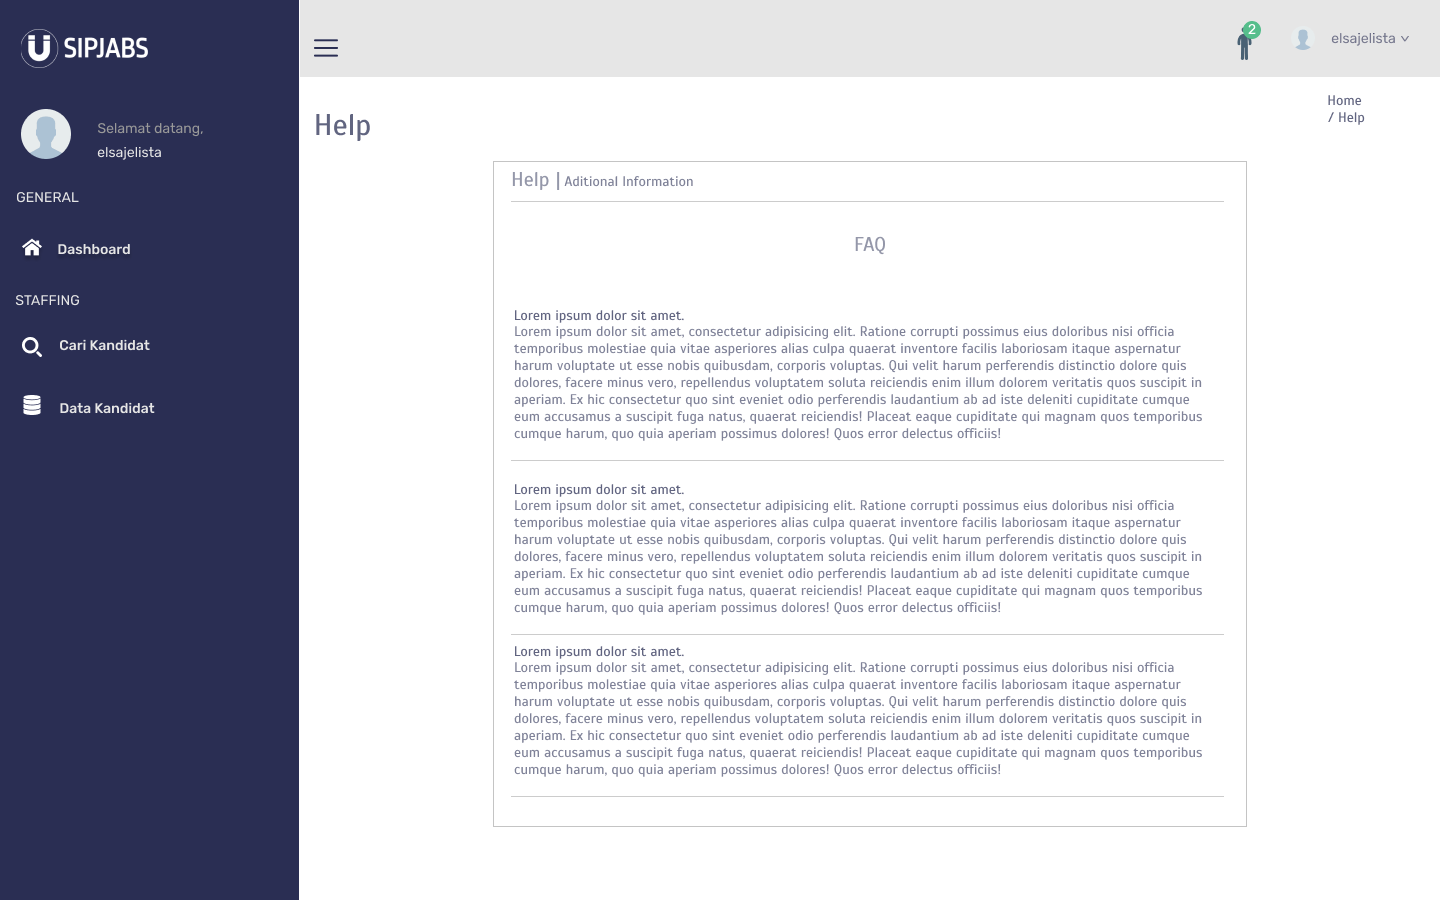
\includegraphics[width=0.6\textwidth, height=60mm]{pics/user/help.png}} 
		& Pada halaman help akan mengenai informasi dari sistem aplikasi ini\\
		
		\hline
		
	\end{tabular}
\end{table}

\begin{table}
	\caption{Tabel Perancangan Antar Muka User (2)}
	\centering
	\begin{tabular}{ | c | c | p{35mm} |}
		\hline 
		\textbf{No} & \textbf{Gambar} &  \textbf{Keterangan} \\ 
		\hline
		
		7. & \raisebox{-\totalheight}{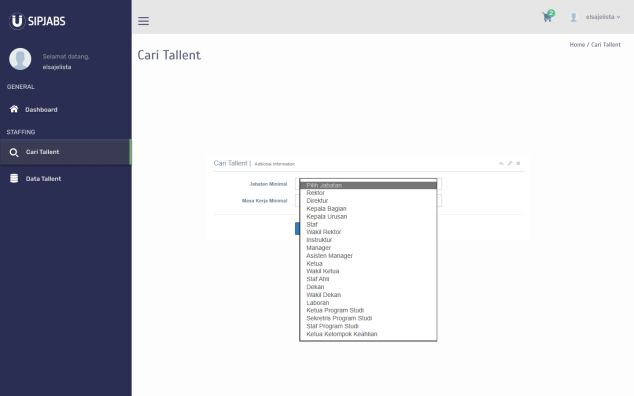
\includegraphics[width=0.6\textwidth, height=60mm]{pics/user/caritallent.png}} 
		& User dapat memilih jabatan dan masa kerja yang diinginkan untuk mengantikan atau mengisi posisi yang kosong.  \\
		
		\hline
		
		8. & \raisebox{-\totalheight}{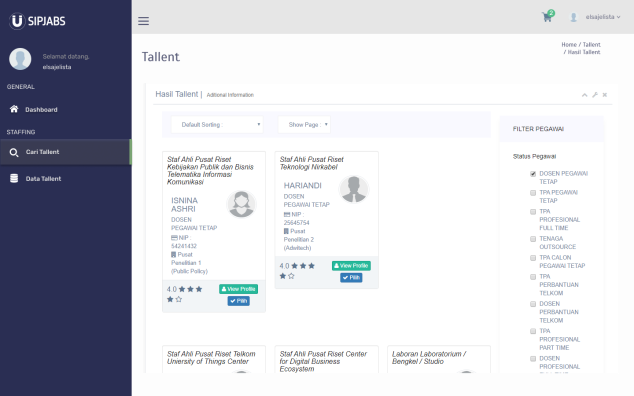
\includegraphics[width=0.6\textwidth, height=60mm]{pics/user/hasiltallent.png}} 
		& Halaman ini akan menampilkan tallent yang sudah di pilih dengan syarat tententu.   \\
		
		\hline
		
		9. & \raisebox{-\totalheight}{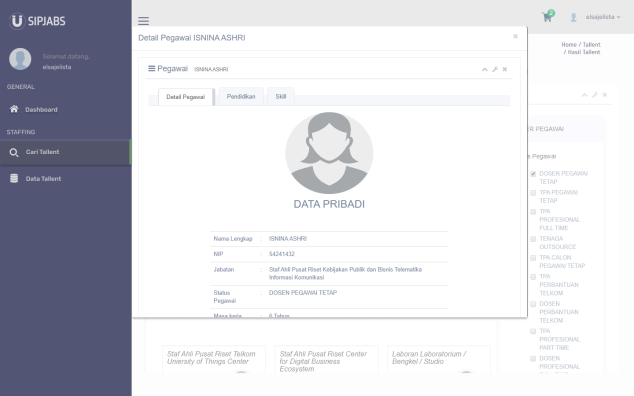
\includegraphics[width=0.6\textwidth, height=60mm]{pics/user/viewdetailtallent.png}} 
		& Halaman ini akan menampilkan data pribadi dari tallent tersebut.\\
		
		\hline
		
	\end{tabular}
\end{table}

\begin{table}
	\caption{Tabel Perancangan Antar Muka User (3)}
	\centering
	\begin{tabular}{ | c | c | p{35mm} |}
		\hline 
		\textbf{No} & \textbf{Gambar} &  \textbf{Keterangan} \\ 
		\hline
		
		10. & \raisebox{-\totalheight}{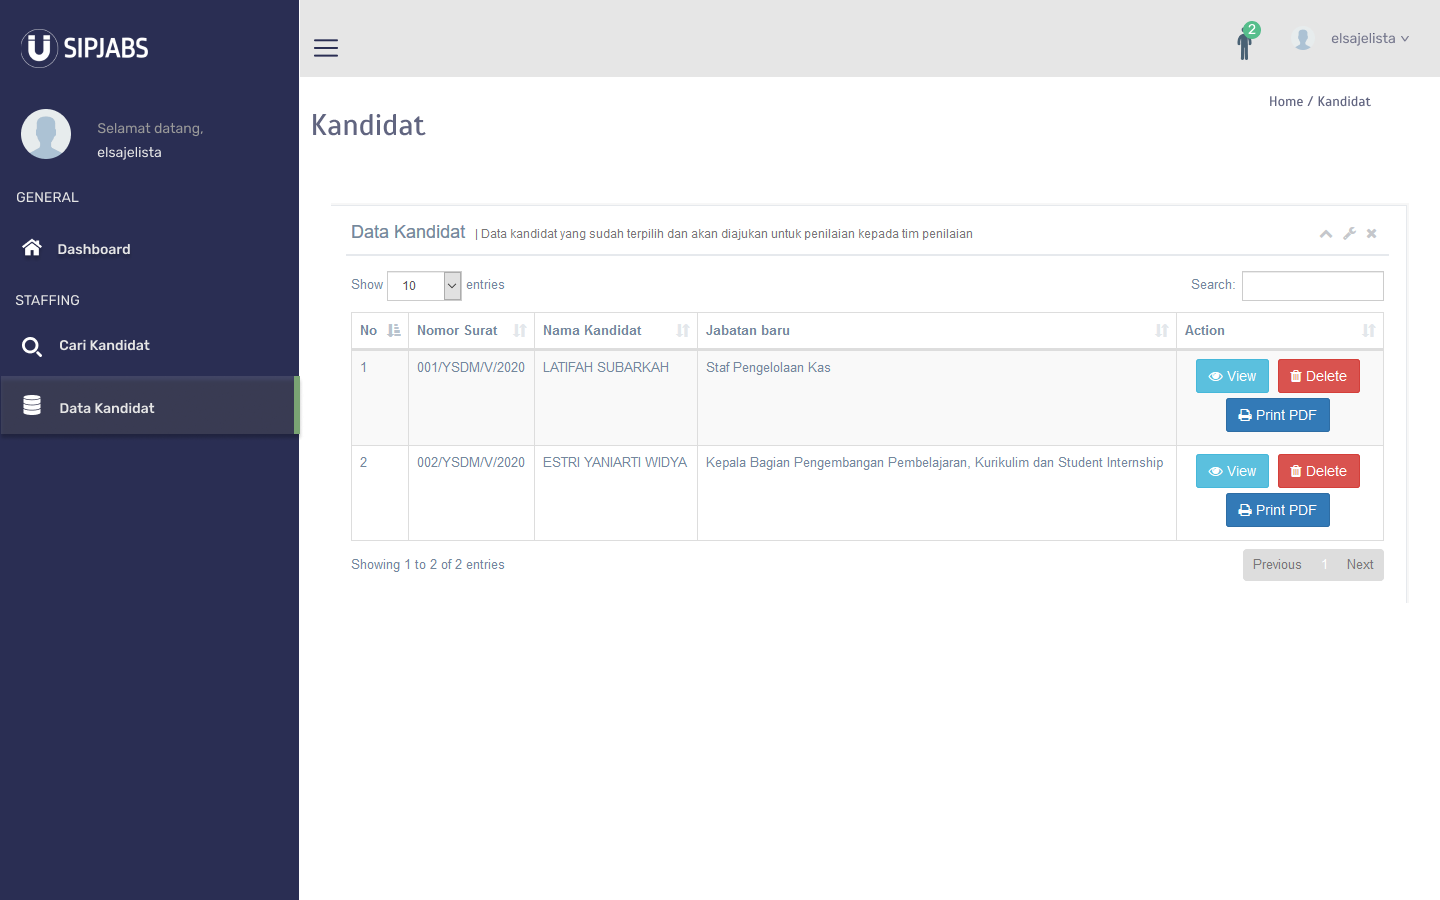
\includegraphics[width=0.6\textwidth, height=60mm]{pics/user/datatallent.png}} 
		& Halaman ini akan menampilkan data tallent yang sudah di proses dari cart tersebut.  \\
		
	
		\hline
		
		11. & \raisebox{-\totalheight}{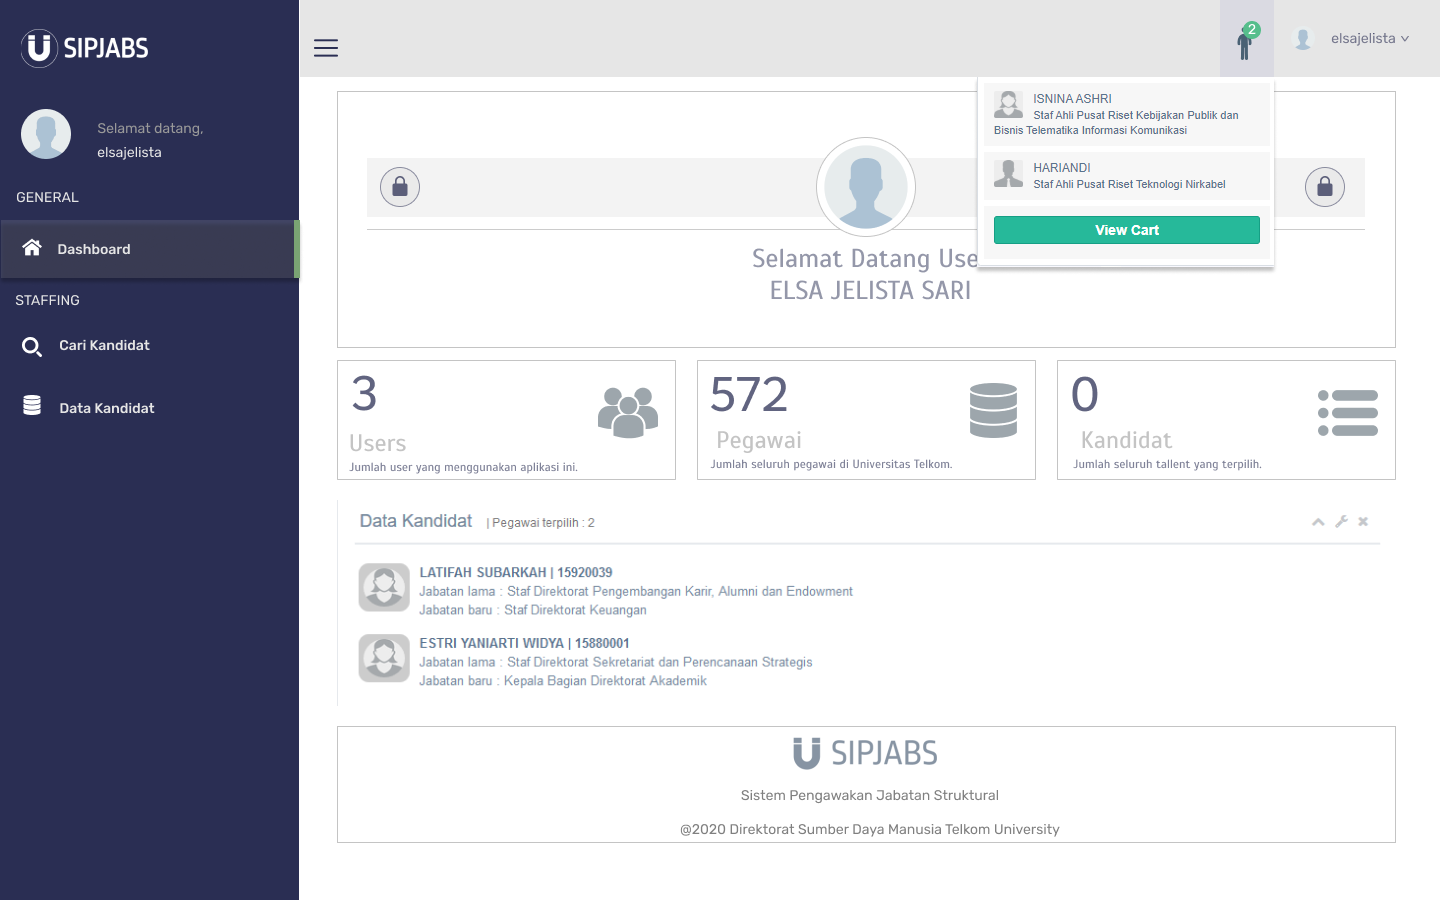
\includegraphics[width=0.6\textwidth, height=60mm]{pics/user/cartuser.png}} 
		& Halaman ini akan menampilkan data tallent yang sudah dipilih dan masih ada kemungkinan bisa di ubah sebelum ditetapkan menjadi tallent.  \\
		
		\hline
		
		12. & \raisebox{-\totalheight}{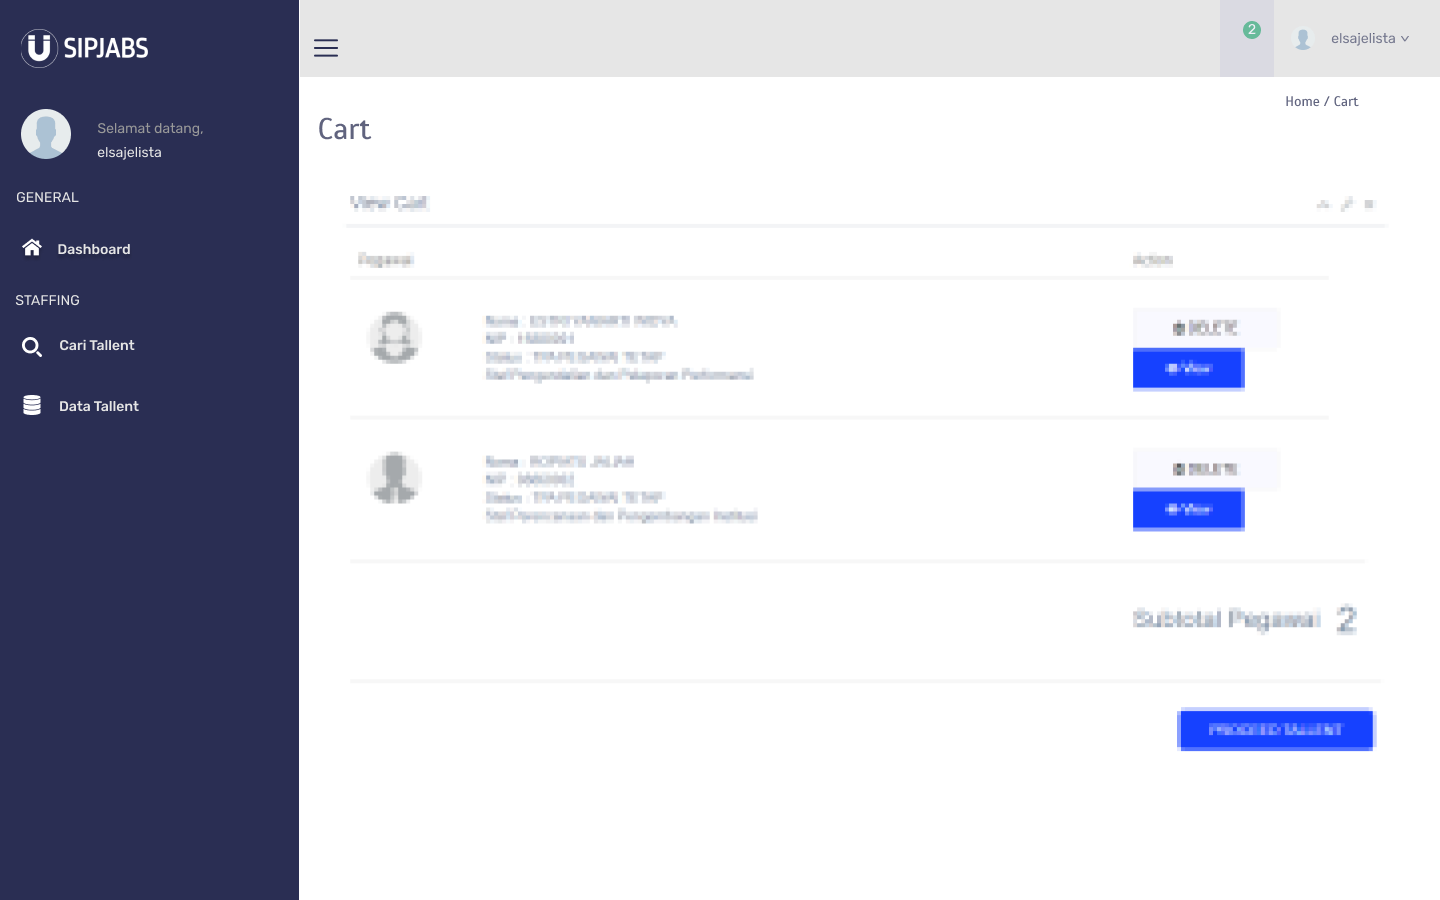
\includegraphics[width=0.6\textwidth, height=60mm]{pics/user/viewcart.png}} 
		& Halaman ini akan menampilkan data tallent yang sudah di pilih dan akan di proses ditetapkan untuk menjadi tallent.  \\
		
		
		\hline
		
	\end{tabular}
\end{table}
\subsection{Perancangan Level Tinggi}

\begin{figure}
	\centering
	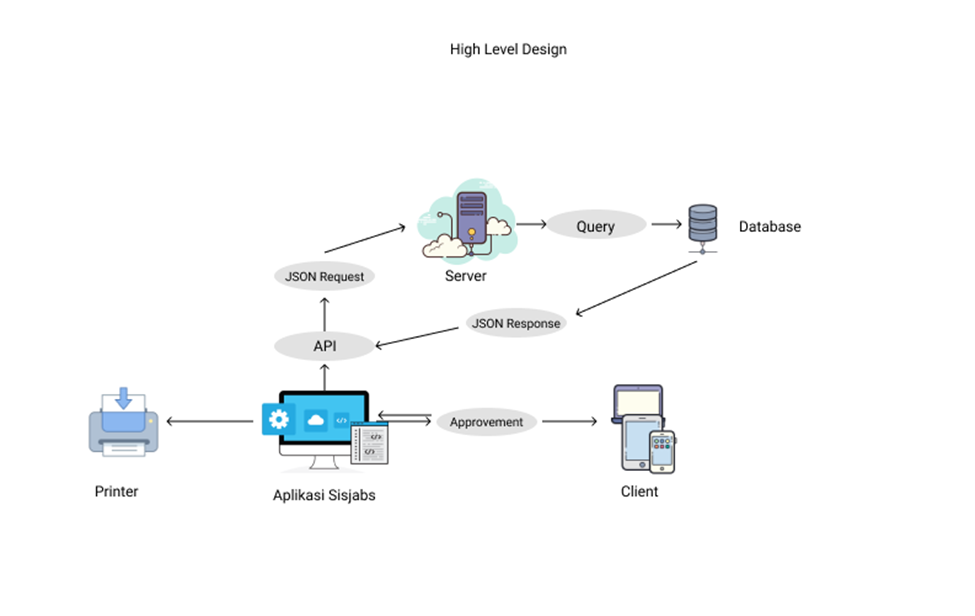
\includegraphics[width=0.9\textwidth]
	{pics/highleveldesign.png}
	\caption{High Level Design}
	\label{fig:34}
\end{figure}

Alur perancanaan level tinggi pada aplikasi pengawakan pegawai dimulai dari pengambilan API dalam bentuk JSON Request ke server. Pengambilan data akan di filter berdasarkan dengan query yang dibuat berdasarkan data yang diperoleh dari database yang ada. Kemudian database akan memberikan umpan balik berupa JSON Response berdasarkan request data yang akan ditampilkan kepada pengguna. 

